% ថ្នាក់ទី ១១ (វិទ្យាសាស្ត្រ) · ជំពូកទី ៤ · មេរៀនទី ៣ · សៀវភៅទំព័រ ១៨៨–២១៧
\chapter{ការបំប្លែងលីនេអ៊ែរ}

\begin{objBox}[វត្ថុបំណង]
\begin{enumerate}[1]
  \item បកស្រាយបំប្លែងលីនេអ៊ែរជាម៉ាទ្រីស
  \item កំណត់រូបភាពតាមការបំប្លែងលីនេអ៊ែរ
  \item កំណត់រូបភាពតាមការបំប្លែងលីនេអ៊ែរបណ្ដាក់
  \item កំណត់រូបភាពតាមការបំប្លែងលីនេអ៊ែរបណ្ដាក់ក្នុងត្រីកោណមាត្រ ។
\end{enumerate}
\end{objBox}

\section{ការបំប្លែងលីនេអ៊ែរ}
\subsection{សញ្ញាណ}

យើងធ្លាប់បានរៀនរួចមកហើយនូវបំប្លែងចំណុចមួយចំនួននៅក្នុងប្លង់ ។

\begin{example}[ឧទាហរណ៍]
បើគេបំប្លែងចំណុច $M(x, y)$ ទៅជា $M'(x', y')$ តាមការបំប្លែង $H$ ដែលមានផ្ចិត $O$ និងផលធៀប $4$ នោះគេបានសមីការ $\begin{cases} x' = 4x\\ y' = 4y \end{cases}$ ។
\end{example}

សមីការនៃការបំប្លែងចាំងដែលសរសេរបែបនេះ ហៅថាសមីការដឺក្រេទី $1$ ឬហៅថា \textbf{សមីការលីនេអ៊ែរ} ។ ក្នុងករណីនេះ គេថាបំប្លែងចាំងជាបំប្លែងលីនេអ៊ែរ ។

\begin{formulaBox}[ជាទូទៅ]
ការបំប្លែងលីនេអ៊ែរដែលបំប្លែងចំណុច $M(x, y)$ ទៅ $M'(x', y')$ កំណត់ដោយសមីការ $x' = ax + cy$, \ $y' = bx + dy$ ។
\end{formulaBox}

ដើម្បីងាយស្រួលសិក្សាទៅមុខ គេអាចបកស្រាយបំប្លែងលីនេអ៊ែរឱ្យមានទម្រង់ជាម៉ាទ្រីស
\[ \begin{bmatrix} x'\\ y' \end{bmatrix} = \begin{bmatrix} a & c\\ b & d \end{bmatrix}\begin{bmatrix} x\\ y \end{bmatrix} \]
ក្នុងករណីនេះគេថា $A = \begin{bmatrix} a & c\\ b & d \end{bmatrix}$ ជាម៉ាទ្រីសនៃបំប្លែងលីនេអ៊ែរ ។ ចំណុច $\begin{bmatrix} x'\\ y' \end{bmatrix}$ ជារូបភាពនៃ $\begin{bmatrix} x\\ y \end{bmatrix}$ តាមការបំប្លែងលីនេអ៊ែរ $A$ ។ គេអាចគណនា $x', y'$ បានដោយគេគុណម៉ាទ្រីស $\begin{bmatrix} a & c\\ b & d \end{bmatrix}$ និង $\begin{bmatrix} x\\ y \end{bmatrix}$ រួចផ្ទឹមតួម៉ាទ្រីសនៃអង្គទី $1$ និងតួម៉ាទ្រីសនៃអង្គទី $2$ ។

\begin{note}[សម្គាល់]
ដើម្បីសម្រួលក្នុងសំណេរ គេអាចប្រើអក្សរ $A$ ដដែលនេះសម្រាប់សម្គាល់ថាជាម៉ាទ្រីសផង និងជាបំប្លែងលីនេអ៊ែរផង ។
\end{note}

\begin{example}[ឧទាហរណ៍ ១]
រូបភាពនៃចំណុច $\left(2, \dfrac{1}{2}\right)$ តាមការបំប្លែង $A = \begin{bmatrix} -\frac{1}{2} & 1\\ 4 & 3 \end{bmatrix}$ គឺ
\[
\begin{aligned}
\begin{bmatrix} x'\\ y' \end{bmatrix} &= \begin{bmatrix} -\frac{1}{2} & 1\\ 4 & 3 \end{bmatrix}\begin{bmatrix} 2\\ \frac{1}{2} \end{bmatrix} = \begin{bmatrix} -\frac{1}{2}\times 2 + 1\times\frac{1}{2}\\[3pt] 4\times 2 + 3\times\frac{1}{2} \end{bmatrix}\\
&= \begin{bmatrix} -\frac{1}{2}\\[3pt] \frac{19}{2} \end{bmatrix}
\end{aligned}
\]
ដូច្នេះ រូបភាពនៃ $\left(2, \dfrac{1}{2}\right)$ គឺ $\left(-\dfrac{1}{2}, \dfrac{19}{2}\right)$ ។
\end{example}

ចំពោះបំប្លែងលីនេអ៊ែរដែលមានម៉ាទ្រីស $I = \begin{bmatrix} 1 & 0\\ 0 & 1 \end{bmatrix}$ រូបភាពវាគឺ
\[ \begin{bmatrix} x'\\ y' \end{bmatrix} = \begin{bmatrix} 1 & 0\\ 0 & 1 \end{bmatrix}\begin{bmatrix} x\\ y \end{bmatrix} = \begin{bmatrix} x + 0\\ 0 + y \end{bmatrix} = \begin{bmatrix} x\\ y \end{bmatrix} \]
គេសង្កេតឃើញថា រូបភាពនៃ $\begin{bmatrix} x'\\ y' \end{bmatrix}$ ត្រួតលើភាពដើម $\begin{bmatrix} x\\ y \end{bmatrix}$ ។ គេថា $I$ ជាបំប្លែងលីនេអ៊ែរដដែល ។ មានន័យថាចំណុចដែលប្លែងដោយ $I$ នៅតែជាចំណុចនោះដដែល ។

\begin{example}[ឧទាហរណ៍ ២]
រូបភាពនៃចំណុច $\left(-\dfrac{1}{2}, 3\right)$ តាម $I = \begin{bmatrix} 1 & 0\\ 0 & 1 \end{bmatrix}$ គឺ
\[ \begin{bmatrix} x'\\ y' \end{bmatrix} = \begin{bmatrix} 1 & 0\\ 0 & 1 \end{bmatrix}\begin{bmatrix} -\frac{1}{2}\\ 3 \end{bmatrix} = \begin{bmatrix} -\frac{1}{2}\\ 3 \end{bmatrix} \]
ដូច្នេះ $x' = -\dfrac{1}{2}$, $y' = 3$ ។
\end{example}

\begin{example}[លំហាត់គំរូ ១]
បង្ហាញថា បើម៉ាទ្រីស $A$ បំប្លែងគ្រប់ចំណុច $M$ នៅតែជាចំណុច $M$ ដដែល នោះម៉ាទ្រីស $A = I$ ។
\end{example}
\ans
តាង $A = \begin{bmatrix} a & c\\ b & d \end{bmatrix}$ ជាម៉ាទ្រីសដែលបំប្លែង $M(x, y)$ ទៅ $M(x, y)$ ដដែល ។ យើងបាន
\[ \begin{bmatrix} x\\ y \end{bmatrix} = \begin{bmatrix} a & c\\ b & d \end{bmatrix}\begin{bmatrix} x\\ y \end{bmatrix} \quad\text{ឬ}\quad \begin{bmatrix} x\\ y \end{bmatrix} = \begin{bmatrix} ax + cy\\ bx + dy \end{bmatrix} \]
យើងបាន $\begin{cases} x = ax + cy\\ y = bx + dy \end{cases}$ ចំពោះគ្រប់ $x, y$ $\Rightarrow \begin{cases} a = 1, \ c = 0\\ b = 0, \ d = 1 \end{cases}$ ។ ដូច្នេះ $A = \begin{bmatrix} 1 & 0\\ 0 & 1 \end{bmatrix} = I$ ។

\begin{example}[លំហាត់គំរូ ២]
កំណត់ម៉ាទ្រីស $A$ ដែលបំប្លែងពីចំណុច $(1, 2)$ ទៅចំណុច $(8, 1)$ និងបំប្លែងពីចំណុច $(-1, 1)$ ទៅ $(1, 2)$ ។
\end{example}
\ans
តាង $A = \begin{bmatrix} a & c\\ b & d \end{bmatrix}$ ជាម៉ាទ្រីសបំប្លែងពីចំណុច $(1, 2)$ ទៅចំណុច $(8, 1)$ នោះយើងបាន
\[ \begin{bmatrix} 8\\ 1 \end{bmatrix} = \begin{bmatrix} a & c\\ b & d \end{bmatrix}\begin{bmatrix} 1\\ 2 \end{bmatrix} \Rightarrow \begin{cases} a + 2c = 8 & (1)\\ b + 2d = 1 & (2) \end{cases} \]
\[ \begin{bmatrix} 1\\ 2 \end{bmatrix} = \begin{bmatrix} a & c\\ b & d \end{bmatrix}\begin{bmatrix} -1\\ 1 \end{bmatrix} \Rightarrow \begin{cases} -a + c = 1 & (3)\\ -b + d = 2 & (4) \end{cases} \]
ដោះស្រាយប្រព័ន្ធសមីការ $(1)$ និង $(3)$ យើងបាន $a = 2$, $c = 3$ ។ ដោះស្រាយប្រព័ន្ធសមីការ $(2)$ និង $(4)$ យើងបាន $b = -1$, $d = 1$ ។

ដូច្នេះ ម៉ាទ្រីសដែលត្រូវរកគឺ $A = \begin{bmatrix} 2 & 3\\ -1 & 1 \end{bmatrix}$ ។

\begin{pro}
\begin{enumerate}[1]
  \item គេប្លែងចំណុច $M(x, y)$ ទៅ $M'(x', y')$ តាមម៉ាទ្រីស $A$ ដែល $x' = x\cos\alpha - y\sin\alpha$, \ $y' = x\sin\alpha + y\cos\alpha$ ។ កំណត់ម៉ាទ្រីស $A$ ។
  \item កំណត់ $\alpha$ ដើម្បីឱ្យចំណុច $M'$ ត្រួតលើ $M$ ។
\end{enumerate}
\ans
\begin{enumerate}[1]
  \item $A = \begin{bmatrix} \cos\alpha & -\sin\alpha\\ \sin\alpha & \cos\alpha \end{bmatrix}$
  \item $\alpha = 2k\pi$, \ $(k \in \mathbb{Z})$ ។
\end{enumerate}
\end{pro}

\subsection{ចំណុចឥតប្រែប្រួល}

\begin{example}[ឧទាហរណ៍]
កំណត់រូបភាពនៃចំណុច $P(3, 2)$ និង $Q(5, 2)$ ដែលបំប្លែងដោយបំប្លែងលីនេអ៊ែរ $A = \begin{bmatrix} 3 & -5\\ 2 & -4 \end{bmatrix}$ ។
\end{example}
\ans
តាមបម្រាប់រូបភាពនៃ $P$ កំណត់ដោយ
\[ \begin{bmatrix} x'\\ y' \end{bmatrix} = \begin{bmatrix} 3 & -5\\ 2 & -4 \end{bmatrix}\begin{bmatrix} 3\\ 2 \end{bmatrix} = \begin{bmatrix} 3\times 3 - 5\times 2\\ 2\times 3 - 4\times 2 \end{bmatrix} = \begin{bmatrix} -1\\ -2 \end{bmatrix} \]
ដូច្នេះ $P'(-1, -2)$ ។ រូបភាពនៃ $Q$ កំណត់ដោយ
\[ \begin{bmatrix} x'\\ y' \end{bmatrix} = \begin{bmatrix} 3 & -5\\ 2 & -4 \end{bmatrix}\begin{bmatrix} 5\\ 2 \end{bmatrix} = \begin{bmatrix} 3\times 5 - 5\times 2\\ 2\times 5 - 4\times 2 \end{bmatrix} = \begin{bmatrix} 5\\ 2 \end{bmatrix} \]
ដូច្នេះ $Q'(5, 2)$ ។

តាមបំប្លែង $A$ រូបភាពនៃ $P(3, 2)$ គឺ $P'(-1, -2)$ ហើយ $Q(5, 2)$ គឺ $Q'(5, 2)$ នោះគេសង្កេតឃើញថា ចំណុច $Q$ មិនផ្លាស់ប្ដូរទីតាំងទៅតាម $A$ នោះទេ ព្រោះរូបភាពរបស់វា $Q'$ នៅតែជាចំណុច $Q$ ដដែល ។ ក្នុងករណីនេះ គេថា $Q$ ជាចំណុចឥតប្រែប្រួលតាមការបំប្លែង $A$ ។

\begin{formulaBox}[ជាទូទៅ]
$Q$ ជាចំណុចឥតប្រែប្រួលតាមការបំប្លែង $A$ កាលណា $A(Q) = Q$ ។
\end{formulaBox}

\begin{itemize}
  \item ចំពោះបំប្លែងចាំង $H(O, k)$ កំណត់ដោយ $x' = kx$, $y' = ky$ ។ គល់ $O$ គឺជាចំណុចឥតប្រែប្រួល ព្រោះ $O(0, 0)$ ផ្ដល់រូបភាព $O(0, 0)$ ដដែល ។
  \item ចំពោះបំប្លែងដែលមានម៉ាទ្រីសឯកតា $I$ គឺ $I = \begin{bmatrix} 1 & 0\\ 0 & 1 \end{bmatrix}$ ។ គ្រប់ចំណុចនៃប្លង់ដែលប្លែងតាម $I$ នៅតែជាចំណុចខ្លួនឯងដដែល ព្រោះ $\begin{bmatrix} x'\\ y' \end{bmatrix} = \begin{bmatrix} 1 & 0\\ 0 & 1 \end{bmatrix}\begin{bmatrix} x\\ y \end{bmatrix} = \begin{bmatrix} x\\ y \end{bmatrix}$ ។
\end{itemize}

\begin{example}[លំហាត់គំរូ ១]
គេប្លែងចំណុច $M(x, y)$ ទៅ $M'(x', y')$ កំណត់ដោយ $\begin{bmatrix} x'\\ y' \end{bmatrix} = \begin{bmatrix} 2 & -1\\ 3 & 4 \end{bmatrix}\begin{bmatrix} x\\ y \end{bmatrix} + \begin{bmatrix} 3\\ -3 \end{bmatrix}$ ។ កំណត់ចំណុចឥតប្រែប្រួល ។
\end{example}
\ans
បើ $M(x, y)$ ជាចំណុចឥតប្រែប្រួល លុះត្រាតែ $x' = x$, $y' = y$
\[
\begin{aligned}
\begin{bmatrix} x\\ y \end{bmatrix} &= \begin{bmatrix} 2 & -1\\ 3 & 4 \end{bmatrix}\begin{bmatrix} x\\ y \end{bmatrix} + \begin{bmatrix} 3\\ -3 \end{bmatrix}\\
&= \begin{bmatrix} 2x - y\\ 3x + 4y \end{bmatrix} + \begin{bmatrix} 3\\ -3 \end{bmatrix} = \begin{bmatrix} 2x - y + 3\\ 3x + 4y - 3 \end{bmatrix}
\end{aligned}
\]
យើងបានប្រព័ន្ធ $\begin{cases} 2x - y + 3 = x\\ 3x + 4y - 3 = y \end{cases}$ ឬ $\begin{cases} x - y = -3\\ 3x + 3y = 3 \end{cases}$ ។ ដោះស្រាយប្រព័ន្ធ យើងបាន $x = -1$, $y = 2$ ។

ដូច្នេះ ចំណុចឥតប្រែប្រួលគឺ $(-1, 2)$ ។

\begin{example}[លំហាត់គំរូ ២]
បង្ហាញថាបន្ទាត់ $y = 2x - 1$ ប្លែងតាមម៉ាទ្រីស $\begin{bmatrix} 3 & -1\\ 4 & -1 \end{bmatrix}$ បានរូបភាពខ្លួនឯងដដែល ។
\end{example}
\ans
យក $M(x, y)$ ប្លែងទៅ $M'(x', y')$ តាមម៉ាទ្រីស $\begin{bmatrix} 3 & -1\\ 4 & -1 \end{bmatrix}$ នោះយើងបាន $\begin{bmatrix} x'\\ y' \end{bmatrix} = \begin{bmatrix} 3 & -1\\ 4 & -1 \end{bmatrix}\begin{bmatrix} x\\ y \end{bmatrix}$ ។

បើ $M$ ជាចំណុចមួយនៃបន្ទាត់ $y = 2x - 1$ នោះ $M$ មានកូអរដោនេ $(a, 2a - 1)$ ។ ដូច្នេះ
\[ \begin{bmatrix} x'\\ y' \end{bmatrix} = \begin{bmatrix} 3 & -1\\ 4 & -1 \end{bmatrix}\begin{bmatrix} a\\ 2a - 1 \end{bmatrix} = \begin{bmatrix} 3a - 2a + 1\\ 4a - 2a + 1 \end{bmatrix} = \begin{bmatrix} a + 1\\ 2a + 1 \end{bmatrix} \]
នោះយើងបាន $x' = a + 1$, $y' = 2a + 1$ ។ ដោយបំបាត់ $a$ យើងបាន $y' = 2x' - 1$ ដែលជារូបភាពនៃបន្ទាត់ $y = 2x - 1$ ។ បន្ទាត់ដើម និងរូបភាពវាមានសមីការដូចគ្នាគឺ $y = 2x - 1$ ។

\begin{pro}
\begin{enumerate}[1]
  \item គេប្លែងចំណុច $M(x, y)$ ទៅ $M'(x', y')$ កំណត់ដោយ ។ កំណត់ចំណុចឥតប្រែប្រួល ។
  \begin{enumerate}[a]
    \item $x' = 2y - 3$, \ $y' = x + 1$
    \item $\begin{bmatrix} x'\\ y' \end{bmatrix} = \begin{bmatrix} 3 & 3\\ -2 & -1 \end{bmatrix}\begin{bmatrix} x\\ y \end{bmatrix} + \begin{bmatrix} -4\\ 2 \end{bmatrix}$
  \end{enumerate}
  \item កំណត់រូបភាពនៃបន្ទាត់ $y = 2x - 3$ ដែលប្លែងតាមម៉ាទ្រីស $\begin{bmatrix} 2 & 1\\ 3 & -1 \end{bmatrix}$ ។ តើបន្ទាត់នេះជារូបភាពខ្លួនឯងដដែលឬទេ?
  \item រកចំណុចឥតប្រែប្រួលតាមការបំប្លែង $\begin{bmatrix} 2 & 1\\ 2 & 3 \end{bmatrix}$ ។
  \item រកចំណុចឥតប្រែប្រួលតាមការបំប្លែង $\begin{bmatrix} 3 & 2\\ 3 & 4 \end{bmatrix}$ ។
\end{enumerate}
\ans
\begin{enumerate}[1]
  \item ក. $(1, 2)$ \quad ខ. $(-1, 2)$
  \item $y = \dfrac{1}{4}x + \dfrac{15}{4}$ (មិនមែនជារូបភាពខ្លួនឯងទេ)
  \item គ្រប់ចំណុចនៃបន្ទាត់ $y = -x$
  \item គ្រប់ចំណុចនៃបន្ទាត់ $y = -x$ ។
\end{enumerate}
\end{pro}

\subsection{ការបំប្លែងលីនេអ៊ែរច្រាស}

\begin{example}[ឧទាហរណ៍]
គេបំប្លែងចំណុច $M(x, y)$ ទៅ $M'(x', y')$ តាមការបំប្លែងចាំងដែលមានម៉ាទ្រីស $H = \begin{bmatrix} k & 0\\ 0 & k \end{bmatrix}$ ដែល $k \ne 0$ ។
\end{example}
គេបាន $\begin{bmatrix} x'\\ y' \end{bmatrix} = \begin{bmatrix} k & 0\\ 0 & k \end{bmatrix}\begin{bmatrix} x\\ y \end{bmatrix} = \begin{bmatrix} kx\\ ky \end{bmatrix}$ នាំឱ្យគេបាន $\begin{cases} x' = kx\\ y' = ky \end{cases}$ ។ គេថា $M'$ ជារូបភាពនៃ $M$ តាមការបំប្លែង $H$ ។

ឥឡូវនេះ គេយក $M$ ជារូបភាពនៃ $M'$ វិញ ហើយក្នុងករណីនេះគេត្រូវគណនា $x, y$ ជាអនុគមន៍នៃ $x'$ និង $y'$ ។ គេបាន $x = \dfrac{1}{k}x'$ និង $y = \dfrac{1}{k}y'$ បកស្រាយសមីការនេះជាម៉ាទ្រីសគឺ
\[ \begin{bmatrix} x\\ y \end{bmatrix} = \begin{bmatrix} \frac{1}{k} & 0\\ 0 & \frac{1}{k} \end{bmatrix}\begin{bmatrix} x'\\ y' \end{bmatrix} \]
នោះគេថា $M$ ជារូបភាពនៃ $M'$ តាមការបំប្លែងចាំង $H^{-1}$ ។ ដូច្នេះ $H^{-1} = \begin{bmatrix} \frac{1}{k} & 0\\ 0 & \frac{1}{k} \end{bmatrix}$ ជាម៉ាទ្រីសច្រាសនៃ $H = \begin{bmatrix} k & 0\\ 0 & k \end{bmatrix}$ ។

\begin{formulaBox}[ជាទូទៅ]
គេប្លែង $M(x, y)$ ទៅ $M'(x', y')$ តាមការបំប្លែង $A = \begin{bmatrix} a & c\\ b & d \end{bmatrix}$ នោះ $M' = A(M)$ ឬ $\begin{bmatrix} x'\\ y' \end{bmatrix} = \begin{bmatrix} a & c\\ b & d \end{bmatrix}\begin{bmatrix} x\\ y \end{bmatrix}$ នាំឱ្យ $\begin{cases} x' = ax + cy\\ y' = bx + dy \end{cases}$ ។
\end{formulaBox}

ដើម្បីកំណត់បំប្លែងច្រាស $A^{-1}$ ដែលប្លែង $M'(x', y')$ ទៅ $M(x, y)$ វិញនោះ គេត្រូវគណនា $(x, y)$ ជាអនុគមន៍នៃ $(x', y')$ ។
\[ \begin{cases} ax + cy = x'\\ bx + dy = y' \end{cases} \quad\text{ឬ}\quad \begin{cases} adx + cdy = dx'\\ -bcx - cdy = -cy' \end{cases} \]
សមមូល $(ad - bc)x = dx' - cy'$ ។ ក្នុងករណី $ad - bc \ne 0$ នាំឱ្យគេបាន
\[
\begin{gathered}
x = \frac{1}{ad - bc}(dx' - cy'),\\
y = \frac{1}{ad - bc}(-bx' + ay')
\end{gathered}
\]
បកស្រាយជាម៉ាទ្រីស គេបាន
\[ \begin{bmatrix} x\\ y \end{bmatrix} = \frac{1}{ad - bc}\begin{bmatrix} d & -c\\ -b & a \end{bmatrix}\begin{bmatrix} x'\\ y' \end{bmatrix} \quad\text{ឬ}\quad M = A^{-1}(M') \]
គេថា $A^{-1}$ ជាបំប្លែងច្រាសដែលមានម៉ាទ្រីសច្រាស $A^{-1} = \dfrac{1}{ad - bc}\begin{bmatrix} d & -c\\ -b & a \end{bmatrix}$ ដែល $ad - bc \ne 0$ ។

\begin{theorem}[ម៉ាទ្រីសច្រាស]
ម៉ាទ្រីសច្រាសនៃ $A = \begin{bmatrix} a & c\\ b & d \end{bmatrix}$ គឺ $A^{-1} = \dfrac{1}{ad - bc}\begin{bmatrix} d & -c\\ -b & a \end{bmatrix}$ ដែល $ad - bc \ne 0$ ។
\end{theorem}

\begin{example}[លំហាត់គំរូ ១]
$L$ ជាបន្ទាត់ដែលមានសមីការ $x + 3y - 3 = 0$ ។ រកបំលាស់ទីនៃ $L$ តាមម៉ាទ្រីស $\begin{bmatrix} 1 & -1\\ 2 & 4 \end{bmatrix}$ ។
\end{example}
\ans
តាង $L'$ ជាបំលាស់ទីនៃ $L : x + 3y - 3 = 0$ តាមម៉ាទ្រីស $\begin{bmatrix} 1 & -1\\ 2 & 4 \end{bmatrix}$ ។ ដើម្បីកំណត់ $L'$ គេត្រូវរកចំណុច $A', B'$ ដែលជារូបភាពរៀងគ្នារបស់ចំណុច $A, B$ នៃបន្ទាត់ $L$ ហើយបំលាស់ទីនៃ $L$ គឺជាបន្ទាត់ដែលកាត់តាមចំណុច $A', B'$ ។

គេយក $A(0, 1)$ និង $B(3, 0)$ ជាចំណុចនៃ $L$ នោះគេបានរូបភាពនៃ $A$ កំណត់ដោយ $\begin{bmatrix} 1 & -1\\ 2 & 4 \end{bmatrix}\begin{bmatrix} 0\\ 1 \end{bmatrix} = \begin{bmatrix} -1\\ 4 \end{bmatrix}$ នាំឱ្យ $A'(-1, 4)$ ។ រូបភាពនៃ $B$ គឺ $\begin{bmatrix} 1 & -1\\ 2 & 4 \end{bmatrix}\begin{bmatrix} 3\\ 0 \end{bmatrix} = \begin{bmatrix} 3\\ 6 \end{bmatrix}$ នាំឱ្យ $B'(3, 6)$ ។

ដូច្នេះ បន្ទាត់ $L'$ កាត់តាមពីរចំណុច $A'$ និង $B'$ កំណត់ដោយសមីការ $L' : x - 2y + 9 = 0$ ។

\begin{center}
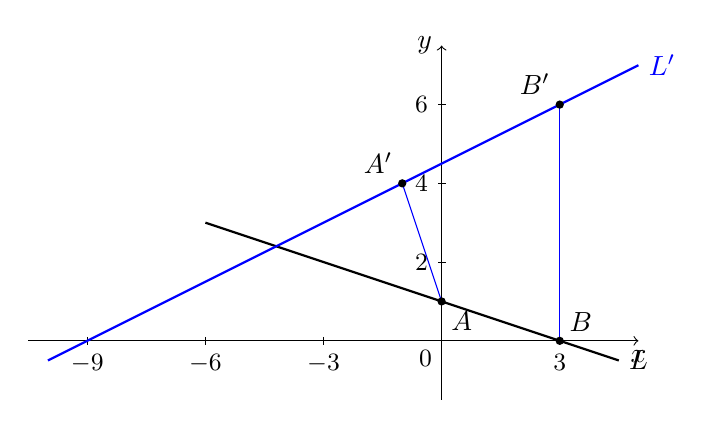
\begin{tikzpicture}[scale=0.5]
  \draw[->] (-10.5,0) -- (5,0) node[below] {$x$};
  \draw[->] (0,-1.5) -- (0,7.5) node[left] {$y$};
  \foreach \x in {-9,-6,-3,3} \draw (\x,0.1) -- (\x,-0.1) node[below] {\small $\x$};
  \foreach \y in {2,4,6} \draw (0.1,\y) -- (-0.1,\y) node[left] {\small $\y$};
  \node[below left] at (0,0) {\small $0$};
  \draw[thick] (-6,3) -- (4.5,-0.5) node[right] {$L$};
  \draw[thick,blue] (-10,-0.5) -- (5,7) node[right] {$L'$};
  \draw[blue] (0,1) -- (-1,4);
  \draw[blue] (3,0) -- (3,6);
  \fill (0,1) circle (3pt) node[below right] {$A$};
  \fill (3,0) circle (3pt) node[above right] {$B$};
  \fill (-1,4) circle (3pt) node[above left] {$A'$};
  \fill (3,6) circle (3pt) node[above left] {$B'$};
\end{tikzpicture}
\end{center}

\begin{formulaBox}[ជាទូទៅ]
ដើម្បីកំណត់រូបភាពនៃបន្ទាត់ $L$ គេត្រូវគណនា $x, y$ ជាអនុគមន៍នៃ $x', y'$ រួចយកទៅជំនួសក្នុងសមីការ $L : x + 3y - 3 = 0$ ។
\end{formulaBox}

បើ $A = \begin{bmatrix} 1 & -1\\ 2 & 4 \end{bmatrix}$ នោះ $A^{-1} = \dfrac{1}{6}\begin{bmatrix} 4 & 1\\ -2 & 1 \end{bmatrix}$ ហើយ
\[ \begin{bmatrix} x\\ y \end{bmatrix} = A^{-1}\begin{bmatrix} x'\\ y' \end{bmatrix} = \frac{1}{6}\begin{bmatrix} 4 & 1\\ -2 & 1 \end{bmatrix}\begin{bmatrix} x'\\ y' \end{bmatrix} = \frac{1}{6}\begin{bmatrix} 4x' + y'\\ -2x' + y' \end{bmatrix} \]
យើងបាន $x = \dfrac{4x' + y'}{6}$, $y = \dfrac{-2x' + y'}{6}$ ។ ជំនួសក្នុងសមីការបន្ទាត់ $L$ ៖
\[
\begin{gathered}
\frac{4x' + y'}{6} + 3\left(\frac{-2x' + y'}{6}\right) - 3 = 0 \quad \text{ឬ}\\
x' - 2y' + 9 = 0
\end{gathered}
\]
ដូច្នេះ បន្ទាត់ $L : x + 3y - 3 = 0$ ផ្លាស់ទីទៅបន្ទាត់ $L' : x - 2y + 9 = 0$ ។

\begin{example}[លំហាត់គំរូ ២]
កំណត់រូបភាពនៃរង្វង់ $C : x^2 + y^2 = 4$ តាម $A = \begin{bmatrix} 3 & 0\\ 0 & 3 \end{bmatrix}$ ។
\end{example}
\ans
$A = \begin{bmatrix} 3 & 0\\ 0 & 3 \end{bmatrix}$ នោះ $A^{-1} = \dfrac{1}{9}\begin{bmatrix} 3 & 0\\ 0 & 3 \end{bmatrix}$ ។
\[ \begin{bmatrix} x\\ y \end{bmatrix} = A^{-1}\begin{bmatrix} x'\\ y' \end{bmatrix} = \frac{1}{9}\begin{bmatrix} 3 & 0\\ 0 & 3 \end{bmatrix}\begin{bmatrix} x'\\ y' \end{bmatrix} = \begin{bmatrix} \frac{1}{3}x'\\[2pt] \frac{1}{3}y' \end{bmatrix} \]
ជំនួស $x, y$ ក្នុងសមីការរង្វង់ ៖ $\left(\dfrac{1}{3}x'\right)^2 + \left(\dfrac{1}{3}y'\right)^2 = 4 \Rightarrow \dfrac{1}{9}x'^2 + \dfrac{1}{9}y'^2 = 4 \Rightarrow x'^2 + y'^2 = 36$ ។

ដូច្នេះ រូបភាពនៃរង្វង់ $x^2 + y^2 = 4$ គឺជារង្វង់ដែលមានសមីការ $x^2 + y^2 = 36$ ។

\begin{center}
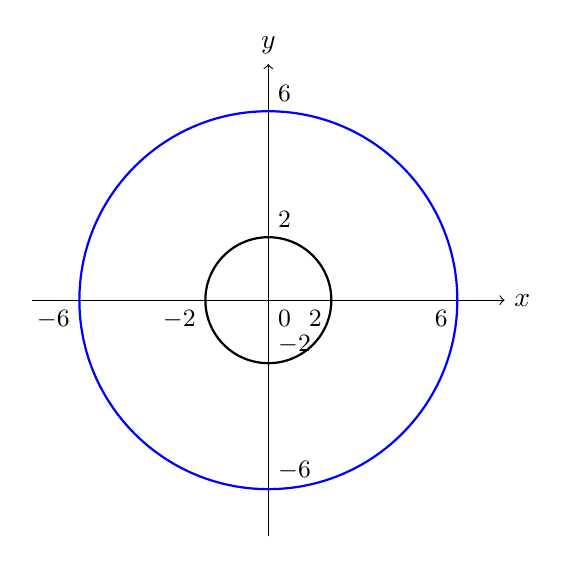
\begin{tikzpicture}[scale=0.4]
  \draw[->] (-7.5,0) -- (7.5,0) node[right] {$x$};
  \draw[->] (0,-7.5) -- (0,7.5) node[above] {$y$};
  \draw[thick] (0,0) circle (2);
  \draw[thick,blue] (0,0) circle (6);
  \foreach \t in {-6,-2,2,6} {\node[below left] at (\t,0) {\small $\t$}; \node[above right] at (0,\t) {\small $\t$};}
  \node[below right] at (0,0) {\small $0$};
\end{tikzpicture}
\end{center}

\begin{example}[លំហាត់គំរូ ៣]
កំណត់រូបភាពនៃសមីការវិចទ័រ $\overrightarrow{r} = \begin{bmatrix} 1\\ 3 \end{bmatrix} + \lambda\begin{bmatrix} -1\\ 4 \end{bmatrix}$ ដែលប្លែងដោយម៉ាទ្រីស $\begin{bmatrix} 2 & 1\\ -1 & 1 \end{bmatrix}$ ។
\end{example}
\ans
ដោយវិចទ័រ $\overrightarrow{r} = \begin{bmatrix} 1\\ 3 \end{bmatrix} + \lambda\begin{bmatrix} -1\\ 4 \end{bmatrix}$ ប្លែងទៅ $\overrightarrow{r}\,' = \overrightarrow{a}\,' + \lambda\overrightarrow{b}\,'$ ។ ក្នុងករណីនេះកូអរដោនេនៃវិចទ័រ $\overrightarrow{a} = \begin{bmatrix} 1\\ 3 \end{bmatrix}$ និង $\overrightarrow{b} = \begin{bmatrix} -1\\ 4 \end{bmatrix}$ ។ ដូច្នេះ
\[
\begin{gathered}
\overrightarrow{a}\,' = \begin{bmatrix} 2 & 1\\ -1 & 1 \end{bmatrix}\begin{bmatrix} 1\\ 3 \end{bmatrix} = \begin{bmatrix} 5\\ 2 \end{bmatrix},\\
\overrightarrow{b}\,' = \begin{bmatrix} 2 & 1\\ -1 & 1 \end{bmatrix}\begin{bmatrix} -1\\ 4 \end{bmatrix} = \begin{bmatrix} 2\\ 5 \end{bmatrix}
\end{gathered}
\]
ដូច្នេះរូបភាពនៃសមីការវិចទ័រគឺ $\overrightarrow{r}\,' = \begin{bmatrix} 5\\ 2 \end{bmatrix} + \lambda\begin{bmatrix} 2\\ 5 \end{bmatrix}$ ។

\begin{pro}
\begin{enumerate}[1]
  \item កំណត់រូបភាពនៃបន្ទាត់ដែលប្លែងដោយម៉ាទ្រីស $\begin{bmatrix} 1 & 2\\ 3 & 4 \end{bmatrix}$ ។
  \begin{tasks}(3)
    \task $y = 2x + 1$
    \task អ័ក្សអាប់ស៊ីស
    \task $2x + y + 1 = 0$
  \end{tasks}
  \item កំណត់រូបភាពនៃបន្ទាត់ $y = 2x - 3$ ដែលប្លែងដោយម៉ាទ្រីស $\begin{bmatrix} 2 & 1\\ 3 & -1 \end{bmatrix}$ ។
  \item កំណត់រូបភាពនៃវិចទ័រ $\overrightarrow{r} = \begin{bmatrix} 1\\ 3 \end{bmatrix} + \lambda\begin{bmatrix} 1\\ 2 \end{bmatrix}$ ដែលប្លែងដោយម៉ាទ្រីស $\begin{bmatrix} 2 & -1\\ -4 & 2 \end{bmatrix}$ ។
\end{enumerate}
\ans
\begin{enumerate}[1]
  \item ក. $y' = \dfrac{11}{5}x' - \dfrac{2}{5}$ \quad ខ. $y' = 3x'$ \quad គ. $5x' - 3y' - 2 = 0$
  \item $y' = \dfrac{1}{4}(x' + 15)$
  \item $\overrightarrow{r}\,' = \begin{bmatrix} -1\\ 2 \end{bmatrix} + \lambda\begin{bmatrix} 0\\ 0 \end{bmatrix}$ គឺបន្ទាត់ទាំងមូលប្លែងទៅចំណុចតែមួយ $(-1, 2)$ ។
\end{enumerate}
\end{pro}

\section{ការបំប្លែងឆ្លុះ}
\subsection{ការបំប្លែងឆ្លុះធៀបនឹងអ័ក្ស \texorpdfstring{$x'x$}{x'x}}

\begin{center}
\begin{tikzpicture}[scale=0.8]
  \draw[->] (-1,0) -- (4,0) node[right] {$x$};
  \draw[->] (0,-2.8) -- (0,2.8) node[above] {$y$};
  \node[below left] at (0,0) {$0$};
  \draw[dashed] (2,2) -- (2,-2);
  \fill (2,2) circle (2pt) node[right] {$M(x, y)$};
  \fill (2,-2) circle (2pt) node[right] {$M'(x', y')$};
  \node[below right] at (2,0) {$H$};
  \draw (2,0.25) -- (2.25,0.25) -- (2.25,0);
\end{tikzpicture}
\end{center}

បើ $M'(x', y')$ ជារូបភាពនៃ $M(x, y)$ តាមការបំប្លែងឆ្លុះធៀបនឹងអ័ក្ស $x'x$ នោះគេបាន $HM' = HM$ ហើយកូអរដោនេនៃចំណុច $x' = x$, $y' = -y$ ។ $M'$ ជារូបភាពនៃ $M$ តាមការបំប្លែងឆ្លុះធៀបនឹងអ័ក្ស $x'x$ គឺ $M \xrightarrow{S_{x'x}} M'$ ។ ក្នុងករណីនេះ គេត្រូវគណនា $(x', y')$ ជាអនុគមន៍នៃ $(x, y)$ ។ តាមការបំប្លែងឆ្លុះធៀបនឹងអ័ក្ស $x'x$ គេបាន ៖
\[ \begin{cases} x' = 1\cdot x + 0\cdot y\\ y' = 0\cdot x + (-1)\cdot y \end{cases} \]
ដើម្បីឱ្យងាយស្រួលសិក្សា គេអាចបកស្រាយបំប្លែងឆ្លុះនេះជាទម្រង់ម៉ាទ្រីសដូចខាងក្រោម ៖ $S_{x'x} : \begin{bmatrix} x'\\ y' \end{bmatrix} = \begin{bmatrix} 1 & 0\\ 0 & -1 \end{bmatrix}\begin{bmatrix} x\\ y \end{bmatrix}$ ។

\begin{formulaBox}[ជាទូទៅ]
ការបំប្លែងលីនេអ៊ែរឆ្លុះធៀបនឹងអ័ក្ស $x'x$ គឺ $S_{x'x} : \begin{bmatrix} x'\\ y' \end{bmatrix} = \begin{bmatrix} 1 & 0\\ 0 & -1 \end{bmatrix}\begin{bmatrix} x\\ y \end{bmatrix}$ ។
\end{formulaBox}

\subsection{ការបំប្លែងឆ្លុះធៀបនឹងអ័ក្ស \texorpdfstring{$y'y$}{y'y}}

\begin{center}
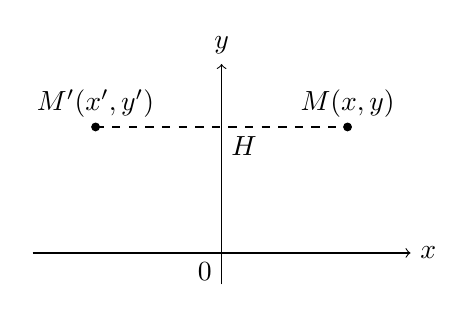
\begin{tikzpicture}[scale=0.8]
  \draw[->] (-3,0) -- (3,0) node[right] {$x$};
  \draw[->] (0,-0.5) -- (0,3) node[above] {$y$};
  \node[below left] at (0,0) {$0$};
  \draw[dashed] (-2,2) -- (2,2);
  \fill (2,2) circle (2pt) node[above] {$M(x, y)$};
  \fill (-2,2) circle (2pt) node[above] {$M'(x', y')$};
  \node[below right] at (0,2) {$H$};
\end{tikzpicture}
\end{center}

បើ $M'(x', y')$ ជារូបភាពនៃ $M(x, y)$ ។ តាមការបំប្លែងឆ្លុះធៀបនឹងអ័ក្ស $y'y$ នោះគេបាន $HM' = HM$ ហើយកូអរដោនេនៃចំណុច $x' = -x$, $y' = y$ ។ $M'$ ជារូបភាពនៃ $M$ តាមការបំប្លែងឆ្លុះធៀបនឹងអ័ក្ស $y'y$ គឺ $M \xrightarrow{S_{y'y}} M'$ ។ ដូច្នេះគេបាន
\[ \begin{cases} x' = (-1)\cdot x + 0\cdot y\\ y' = 0\cdot x + y \end{cases} \]
ដើម្បីឱ្យងាយស្រួលសិក្សា គេអាចបកស្រាយបំប្លែងឆ្លុះនេះជាទម្រង់ម៉ាទ្រីសដូចខាងក្រោម ៖ $S_{y'y} : \begin{bmatrix} x'\\ y' \end{bmatrix} = \begin{bmatrix} -1 & 0\\ 0 & 1 \end{bmatrix}\begin{bmatrix} x\\ y \end{bmatrix}$ ។

\begin{formulaBox}[ជាទូទៅ]
ការបំប្លែងលីនេអ៊ែរឆ្លុះធៀបនឹងអ័ក្ស $y'y$ គឺ $S_{y'y} : \begin{bmatrix} x'\\ y' \end{bmatrix} = \begin{bmatrix} -1 & 0\\ 0 & 1 \end{bmatrix}\begin{bmatrix} x\\ y \end{bmatrix}$ ។
\end{formulaBox}

\subsection{ការបំប្លែងឆ្លុះធៀបនឹងគល់ \texorpdfstring{$O$}{O}}

\begin{center}
\begin{tikzpicture}[scale=0.8]
  \draw[->] (-3,0) -- (3,0) node[right] {$x$};
  \draw[->] (0,-2.5) -- (0,2.5) node[above] {$y$};
  \node[below right] at (0,0) {$0$};
  \draw (-2,-1.6) -- (2,1.6);
  \fill (2,1.6) circle (2pt) node[above] {$M(x, y)$};
  \fill (-2,-1.6) circle (2pt) node[below] {$M'(x', y')$};
\end{tikzpicture}
\end{center}

បើ $M'(x', y')$ ជារូបភាពនៃ $M(x, y)$ តាមការបំប្លែងឆ្លុះធៀបនឹងគល់ $O$ ។ នោះគេបាន $OM' = OM$ ហើយកូអរដោនេនៃចំណុច $x' = -x$, $y' = -y$ ។ $M'$ ជារូបភាពនៃ $M$ តាមការបំប្លែងឆ្លុះធៀបនឹងគល់ $O$ គឺ $M \xrightarrow{S_O} M'$ ។ ដូច្នេះគេបាន
\[ \begin{cases} x' = (-1)\cdot x + 0\cdot y\\ y' = 0\cdot x + (-1)\cdot y \end{cases} \]
គេអាចបកស្រាយបំប្លែងឆ្លុះនេះជាទម្រង់ម៉ាទ្រីស ៖ $S_O : \begin{bmatrix} x'\\ y' \end{bmatrix} = \begin{bmatrix} -1 & 0\\ 0 & -1 \end{bmatrix}\begin{bmatrix} x\\ y \end{bmatrix}$ ។

\begin{formulaBox}[ជាទូទៅ]
ការបំប្លែងលីនេអ៊ែរឆ្លុះធៀបនឹងគល់ $O$ គឺ $S_O : \begin{bmatrix} x'\\ y' \end{bmatrix} = \begin{bmatrix} -1 & 0\\ 0 & -1 \end{bmatrix}\begin{bmatrix} x\\ y \end{bmatrix}$ ។
\end{formulaBox}

\begin{example}[លំហាត់គំរូ]
\begin{enumerate}[a]
  \item បំប្លែងបន្ទាត់ $ax + by + c = 0$ \ $(b \ne 0)$ តាមការបំប្លែងឆ្លុះ $S_{y'y}$ ។
  \item បំប្លែងប៉ារ៉ាបូល $y = (x + 1)^2$ តាមការបំប្លែងឆ្លុះ $S_{x'x}$ ។
\end{enumerate}
\end{example}
\ans
\begin{enumerate}[a]
  \item ដោយ $ax + by + c = 0$ នាំឱ្យ $by = -(ax + c)$ នោះ $y = -\left(\dfrac{a}{b}x + \dfrac{c}{b}\right)$ ។ តាងកូអរដោនេ $\left(k, -\dfrac{a}{b}k - \dfrac{c}{b}\right)$ នៅលើបន្ទាត់ $ax + by + c = 0$ នោះគេបានបំប្លែងបន្ទាត់តាមការបំប្លែងឆ្លុះ $S_{y'y}$ គឺ
  \[ S_{y'y} : \begin{bmatrix} x'\\ y' \end{bmatrix} = \begin{bmatrix} -1 & 0\\ 0 & 1 \end{bmatrix}\begin{bmatrix} k\\ -\frac{a}{b}k - \frac{c}{b} \end{bmatrix} = \begin{bmatrix} -k\\ -\frac{a}{b}k - \frac{c}{b} \end{bmatrix} \]
  នាំឱ្យ $x' = -k$, $y' = -\dfrac{a}{b}k - \dfrac{c}{b}$ នោះ $y' = \dfrac{a}{b}x' - \dfrac{c}{b}$ ។ គេបាន $-ax + by + c = 0$ ។
  \item ដោយ $y = (x + 1)^2$ នោះ $y = x^2 + 2x + 1$ ។ តាងកូអរដោនេ $(m, m^2 + 2m + 1)$ នៅលើប៉ារ៉ាបូល $y = (x + 1)^2$ នោះគេបានបំប្លែងប៉ារ៉ាបូលតាមការបំប្លែងឆ្លុះ $S_{x'x}$ គឺ ៖
  \[
\begin{aligned}
S_{x'x} : \begin{bmatrix} x'\\ y' \end{bmatrix} &= \begin{bmatrix} 1 & 0\\ 0 & -1 \end{bmatrix}\begin{bmatrix} m\\ m^2 + 2m + 1 \end{bmatrix}\\
&= \begin{bmatrix} m\\ -m^2 - 2m - 1 \end{bmatrix}
\end{aligned}
\]
  នាំឱ្យ $x' = m$, $y' = -m^2 - 2m - 1$ នោះ $y' = -x'^2 - 2x' - 1 = -(x' + 1)^2$ នាំឱ្យ $y = -(x + 1)^2$ ។
\end{enumerate}

\begin{pro}
\begin{enumerate}[a]
  \item បំប្លែងបន្ទាត់ $2x + 3y - 6 = 0$ តាមការបំប្លែងឆ្លុះ $S_{y'y}$ និង $S_{x'x}$ ។
  \item បំប្លែងប៉ារ៉ាបូល $y = (x - 1)^2$ តាមការបំប្លែងឆ្លុះ $S_{x'x}$ និង $S_{y'y}$ ។
  \item កំណត់រូបភាពនៃចំណុច $A(2, 3)$ និង $B(-2, -5)$ តាមការបំប្លែងឆ្លុះ $S_{x'x}$, $S_{y'y}$ និង $S_O$ ។
\end{enumerate}
\ans
\begin{enumerate}[a]
  \item $2x - 3y + 6 = 0$ ជារូបភាពតាមការបំប្លែងឆ្លុះធៀប $y'y$ ។ \ $2x - 3y - 6 = 0$ ជារូបភាពតាមការបំប្លែងឆ្លុះធៀប $x'x$ ។
  \item $y = -(x - 1)^2$ ជារូបភាពតាម $S_{x'x}$ ។ \ $y = (x + 1)^2$ ជារូបភាពតាម $S_{y'y}$ ។
  \item តាម $S_{x'x}$ ៖ $A'(2, -3)$, $B'(-2, 5)$ ។ តាម $S_{y'y}$ ៖ $A'(-2, 3)$, $B'(2, -5)$ ។ តាម $S_O$ ៖ $A'(-2, -3)$, $B'(2, 5)$ ។
\end{enumerate}
\end{pro}

\section{ការបំប្លែងចាំង}

បើ $M'(x', y')$ ជារូបភាពនៃ $M(x, y)$ តាមការបំប្លែងចាំង $H$ ដែលមានផលធៀប $k$ ដែល $k \ne 0$ នោះគេបានកូអរដោនេ $x' = kx$, $y' = ky$ អាចសរសេរជា $\begin{cases} x' = kx + 0\cdot y\\ y' = 0\cdot x + ky \end{cases}$ ។ ដើម្បីឱ្យងាយស្រួលសិក្សា គេអាចបកស្រាយបំប្លែងចាំង $H$ នោះជាទម្រង់ម៉ាទ្រីសដូច្នេះ ៖
\[ H(O, k) : \begin{bmatrix} x'\\ y' \end{bmatrix} = \begin{bmatrix} k & 0\\ 0 & k \end{bmatrix}\begin{bmatrix} x\\ y \end{bmatrix} \]
បើ $k = 1$ នោះ $H = \begin{bmatrix} 1 & 0\\ 0 & 1 \end{bmatrix}$ ។ បើ $k = -1$ នោះ $H = \begin{bmatrix} -1 & 0\\ 0 & -1 \end{bmatrix}$ ។

\begin{formulaBox}[ជាទូទៅ]
ការបំប្លែងចាំង $H$ ដែលមានផលធៀប $k$ គឺ $H(O, k) : \begin{bmatrix} x'\\ y' \end{bmatrix} = \begin{bmatrix} k & 0\\ 0 & k \end{bmatrix}\begin{bmatrix} x\\ y \end{bmatrix}$ ។
\end{formulaBox}

\begin{example}[លំហាត់គំរូ]
កំណត់រូបភាពនៃចំណុច $A(2, 4)$, $B\left(\dfrac{1}{2}, -\dfrac{1}{2}\right)$ តាមការបំប្លែងចាំង $H(O, 2)$ និង $H(O, -1)$ ។
\end{example}
\ans
\begin{itemize}
  \item ចំណុច $A(2, 4)$ ៖ $H(O, 2) : \begin{bmatrix} x'\\ y' \end{bmatrix} = \begin{bmatrix} 2 & 0\\ 0 & 2 \end{bmatrix}\begin{bmatrix} 2\\ 4 \end{bmatrix} = \begin{bmatrix} 4\\ 8 \end{bmatrix}$ ។ \ $H(O, -1) : \begin{bmatrix} x'\\ y' \end{bmatrix} = \begin{bmatrix} -1 & 0\\ 0 & -1 \end{bmatrix}\begin{bmatrix} 2\\ 4 \end{bmatrix} = \begin{bmatrix} -2\\ -4 \end{bmatrix}$ ។
  \item ចំណុច $B\left(\dfrac{1}{2}, -\dfrac{1}{2}\right)$ ៖ $H(O, 2) : \begin{bmatrix} x'\\ y' \end{bmatrix} = \begin{bmatrix} 2 & 0\\ 0 & 2 \end{bmatrix}\begin{bmatrix} \frac{1}{2}\\ -\frac{1}{2} \end{bmatrix} = \begin{bmatrix} 1\\ -1 \end{bmatrix}$ ។ \ $H(O, -1) : \begin{bmatrix} x'\\ y' \end{bmatrix} = \begin{bmatrix} -1 & 0\\ 0 & -1 \end{bmatrix}\begin{bmatrix} \frac{1}{2}\\ -\frac{1}{2} \end{bmatrix} = \begin{bmatrix} -\frac{1}{2}\\ \frac{1}{2} \end{bmatrix}$ ។
\end{itemize}

\begin{pro}
\begin{enumerate}[a]
  \item បំប្លែងបន្ទាត់ $ax + by + c = 0$ តាមការបំប្លែងចាំង $H(O, 1)$ និង $H(O, -1)$ ។
  \item បំប្លែងប៉ារ៉ាបូល $y = x^2$ តាមការបំប្លែងចាំង $H(O, 1)$ និង $H(O, -1)$ ។
\end{enumerate}
\ans
\begin{enumerate}[a]
  \item តាម $H(O, 1)$ ៖ $ax + by + c = 0$ (ដដែល) ។ តាម $H(O, -1)$ ៖ $ax + by - c = 0$ ។
  \item តាម $H(O, 1)$ ៖ $y = x^2$ (ដដែល) ។ តាម $H(O, -1)$ ៖ $y = -x^2$ ។
\end{enumerate}
\end{pro}

\section{ការបំប្លែងវិល}

\begin{center}
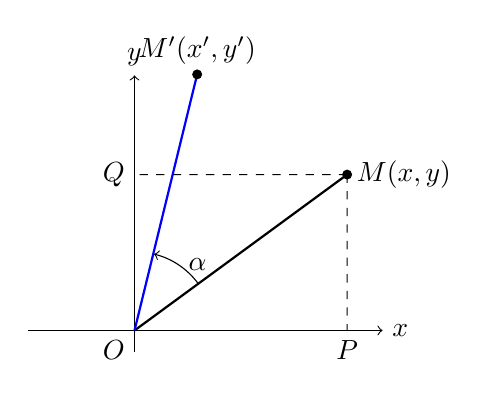
\begin{tikzpicture}[scale=0.9]
  \draw[->] (-1.5,0) -- (3.5,0) node[right] {$x$};
  \draw[->] (0,-0.3) -- (0,3.6) node[above] {$y$};
  \node[below left] at (0,0) {$O$};
  \coordinate (M) at (3,2.2);
  \coordinate (Mp) at ({3*cos(40)-2.2*sin(40)},{3*sin(40)+2.2*cos(40)});
  \draw[thick] (0,0) -- (M);
  \draw[thick,blue] (0,0) -- (Mp);
  \draw[dashed] (M) -- (3,0) node[below] {$P$};
  \draw[dashed] (M) -- (0,2.2) node[left] {$Q$};
  \draw[->] (0.9,{0.9*2.2/3}) arc ({atan(2.2/3)}:{atan(2.2/3)+40}:1.1) node[midway,right] {$\alpha$};
  \fill (M) circle (2pt) node[right] {$M(x, y)$};
  \fill (Mp) circle (2pt) node[above] {$M'(x', y')$};
\end{tikzpicture}
\end{center}

បើ $M'(x', y')$ ជារូបភាពនៃ $M(x, y)$ តាមការបំប្លែងវិល $\mathfrak{R}(O, \alpha)$ នោះគេបាន $OM' = OM$, \ $(\overrightarrow{OM}, \overrightarrow{OM'}) = \alpha$ ។ គេនឹងបកស្រាយបំប្លែងវិលជាសមីការ ។

ដើម្បីគណនា $x', y'$ ជាអនុគមន៍នៃ $x, y$ គេត្រូវ ដៅ $P$ និង $Q$ ជាចំណោលកែងរៀងគ្នានៃ $M$ មកលើអ័ក្ស $\overrightarrow{ox}$ និង $\overrightarrow{oy}$ ។ បើ $M$ ផ្លាស់ទីមក $M'$ តាមមុំ $\alpha$ នោះ $P$ និង $Q$ ក៏ផ្លាស់ទីរៀងគ្នាមក $P'$ និង $Q'$ តាមមុំ $\alpha$ ដែរ ។ ឥឡូវគេគណនាកូអរដោនេនៃចំណុច $P'$ និង $Q'$ ។ តាមរូបបើគេយកកូអរដោនេ $P'(x\cos\alpha, x\sin\alpha)$, \ $Q'(-y\sin\alpha, y\cos\alpha)$ ។

ចំពោះចតុកោណ $OP'M'Q'$ គេមាន $\overrightarrow{OM'} = \overrightarrow{OP'} + \overrightarrow{OQ'}$ ។ $\overrightarrow{OM'} = x'\overrightarrow{i} + y'\overrightarrow{j}$ និង $\overrightarrow{OP'} + \overrightarrow{OQ'} = (x\cos\alpha\,\overrightarrow{i} + x\sin\alpha\,\overrightarrow{j}) + (-y\sin\alpha\,\overrightarrow{i} + y\cos\alpha\,\overrightarrow{j})$
\[ x'\overrightarrow{i} + y'\overrightarrow{j} = (x\cos\alpha - y\sin\alpha)\overrightarrow{i} + (x\sin\alpha + y\cos\alpha)\overrightarrow{j} \]
គេទាញបាន ៖ $x' = x\cos\alpha - y\sin\alpha$, \ $y' = x\sin\alpha + y\cos\alpha$ ។

ក្នុងករណី $\alpha = 60^\circ$ សមីការទៅជា $x' = \dfrac{1}{2}x - \dfrac{\sqrt{3}}{2}y$, \ $y' = \dfrac{\sqrt{3}}{2}x + \dfrac{1}{2}y$ ។ បំប្លែងវិលបកស្រាយដោយសមីការដឺក្រេទី $1$ ជាបំប្លែងលីនេអ៊ែរ ។ គេអាចសរសេរជាទម្រង់ម៉ាទ្រីស
\[ \begin{bmatrix} x'\\ y' \end{bmatrix} = \begin{bmatrix} \frac{1}{2} & -\frac{\sqrt{3}}{2}\\[3pt] \frac{\sqrt{3}}{2} & \frac{1}{2} \end{bmatrix}\begin{bmatrix} x\\ y \end{bmatrix} \]

\begin{formulaBox}[ជាទូទៅ]
ការបំប្លែងវិលនៃមុំ $\alpha$ កំណត់ដោយ $\begin{bmatrix} x'\\ y' \end{bmatrix} = \begin{bmatrix} \cos\alpha & -\sin\alpha\\ \sin\alpha & \cos\alpha \end{bmatrix}\begin{bmatrix} x\\ y \end{bmatrix}$ ។
\end{formulaBox}

\begin{example}[ឧទាហរណ៍]
រូបភាពនៃចំណុច $(-1, 3)$ តាមការបំប្លែងវិល $\mathfrak{R}(O, 60^\circ)$ កំណត់ដោយ
\[ \begin{aligned} \begin{bmatrix} x'\\ y' \end{bmatrix} &= \begin{bmatrix} \cos 60^\circ & -\sin 60^\circ\\ \sin 60^\circ & \cos 60^\circ \end{bmatrix}\begin{bmatrix} -1\\ 3 \end{bmatrix} = \begin{bmatrix} \frac{1}{2} & -\frac{\sqrt{3}}{2}\\[3pt] \frac{\sqrt{3}}{2} & \frac{1}{2} \end{bmatrix}\begin{bmatrix} -1\\ 3 \end{bmatrix}\\ &= \begin{bmatrix} -\frac{1}{2} - \frac{3\sqrt{3}}{2}\\[3pt] -\frac{\sqrt{3}}{2} + \frac{3}{2} \end{bmatrix} = \begin{bmatrix} \frac{-1 - 3\sqrt{3}}{2}\\[3pt] \frac{3 - \sqrt{3}}{2} \end{bmatrix} \end{aligned} \]
\end{example}

\begin{itemize}
  \item ករណី $\alpha = 180^\circ$ នោះ $\mathfrak{R} = \begin{bmatrix} -1 & 0\\ 0 & -1 \end{bmatrix} = S_O$ ។ កាលណាមុំនៃការបំប្លែងវិលស្មើនឹង $180^\circ$ នោះបំប្លែងវិលជាបំប្លែងឆ្លុះធៀបនឹងគល់ $O$ ។
  \item ករណី $\alpha = 360^\circ$ នោះ $\mathfrak{R} = \begin{bmatrix} 1 & 0\\ 0 & 1 \end{bmatrix} = I$ ។ កាលណាមុំនៃការបំប្លែងវិលស្មើនឹង $360^\circ$ នោះបំប្លែងវិលជាបំប្លែងដដែល ក្នុងករណីនេះរូបភាព $M'$ ត្រួតលើធាតុ $M$ ។
  \item បំប្លែងវិលមានម៉ាទ្រីសច្រាស $\mathfrak{R}^{-1} = \begin{bmatrix} \cos\alpha & \sin\alpha\\ -\sin\alpha & \cos\alpha \end{bmatrix}$ ព្រោះដេទែរមីណង់វា $\cos^2\alpha + \sin^2\alpha = 1$ ។
\end{itemize}

\begin{center}
\begin{tikzpicture}[scale=0.7]
  \begin{scope}
  \draw[->] (-3,0) -- (3,0) node[right] {$x$};
  \draw[->] (0,-3) -- (0,3) node[above] {$y$};
  \draw (-2,-1.8) -- (2,1.8);
  \fill (2,1.8) circle (2.5pt) node[above] {$M$};
  \fill (-2,-1.8) circle (2.5pt) node[left] {$M'$};
  \draw[->,blue] ({1.6*cos(42)},{1.6*sin(42)}) arc (42:222:1.6);
  \node[blue] at (-1.6,1.4) {\small $180^\circ$};
  \end{scope}
  \begin{scope}[xshift=8cm]
  \draw[->] (-3,0) -- (3,0) node[right] {$x$};
  \draw[->] (0,-3) -- (0,3) node[above] {$y$};
  \draw (0,0) -- (2,1.8);
  \fill (2,1.8) circle (2.5pt) node[above right] {$M \equiv M'$};
  \draw[->,blue] ({1.6*cos(42)},{1.6*sin(42)}) arc (42:400:1.6);
  \node[blue] at (1.4,-1.6) {\small $360^\circ$};
  \end{scope}
\end{tikzpicture}
\end{center}

\begin{example}[លំហាត់គំរូ ១]
កំណត់រូបភាពនៃចំណុច $(2, \sqrt{3})$ តាមការបំប្លែងវិល $\mathfrak{R}(O, 30^\circ)$ ។
\end{example}
\ans
ម៉ាទ្រីសនៃការបំប្លែងវិលតាមមុំ $30^\circ$ ៖
\[
\begin{aligned}
\begin{bmatrix} \cos\alpha & -\sin\alpha\\ \sin\alpha & \cos\alpha \end{bmatrix} &= \begin{bmatrix} \cos 30^\circ & -\sin 30^\circ\\ \sin 30^\circ & \cos 30^\circ \end{bmatrix}\\
&= \begin{bmatrix} \frac{\sqrt{3}}{2} & -\frac{1}{2}\\[3pt] \frac{1}{2} & \frac{\sqrt{3}}{2} \end{bmatrix}
\end{aligned}
\]
រូបភាពនៃចំណុច $(2, \sqrt{3})$ តាម $\mathfrak{R}$ កំណត់ដោយ
\[
\begin{aligned}
\begin{bmatrix} x'\\ y' \end{bmatrix} &= \begin{bmatrix} \frac{\sqrt{3}}{2} & -\frac{1}{2}\\[3pt] \frac{1}{2} & \frac{\sqrt{3}}{2} \end{bmatrix}\begin{bmatrix} 2\\ \sqrt{3} \end{bmatrix}\\
&= \begin{bmatrix} \frac{\sqrt{3}}{2}\cdot 2 - \frac{1}{2}\sqrt{3}\\[3pt] \frac{1}{2}\cdot 2 + \frac{\sqrt{3}}{2}\cdot\sqrt{3} \end{bmatrix} = \begin{bmatrix} \frac{\sqrt{3}}{2}\\[3pt] \frac{5}{2} \end{bmatrix}
\end{aligned}
\]

\begin{example}[លំហាត់គំរូ ២]
កំណត់រូបភាពនៃបន្ទាត់ $D : y = 2x - 1$ តាមការបំប្លែង $\mathfrak{R}(O, 45^\circ)$ ។
\end{example}
\ans
ម៉ាទ្រីសនៃការបំប្លែងវិលតាមមុំ $45^\circ$ ៖ $\begin{bmatrix} \cos 45^\circ & -\sin 45^\circ\\ \sin 45^\circ & \cos 45^\circ \end{bmatrix} = \begin{bmatrix} \frac{\sqrt{2}}{2} & -\frac{\sqrt{2}}{2}\\[3pt] \frac{\sqrt{2}}{2} & \frac{\sqrt{2}}{2} \end{bmatrix}$ ។

រូបភាពនៃ $D$ តាម $\mathfrak{R}$ តាងដោយ $D'$ ។ ដើម្បីកំណត់ $D'$ គេត្រូវជ្រើសរើសយក $A$ និង $B$ នៃបន្ទាត់ $D$ រួចកំណត់រក $A'$ និង $B'$ ។ បន្ទាត់ដែលកាត់តាម $A'$ និង $B'$ គឺជារូបភាពនៃ $D$ ។ ចំណុច $A(1, 1)$ និង $B(2, 3)$ ផ្ទៀងផ្ទាត់សមីការបន្ទាត់ $y = 2x - 1$ នោះរូបភាពនៃ $A'$ និង $B'$ កំណត់ដោយ
\[ A' = \begin{bmatrix} \frac{\sqrt{2}}{2} & -\frac{\sqrt{2}}{2}\\[3pt] \frac{\sqrt{2}}{2} & \frac{\sqrt{2}}{2} \end{bmatrix}\begin{bmatrix} 1\\ 1 \end{bmatrix} = \begin{bmatrix} 0\\ \sqrt{2} \end{bmatrix} \]
\[
\begin{aligned}
B' &= \begin{bmatrix} \frac{\sqrt{2}}{2} & -\frac{\sqrt{2}}{2}\\[3pt] \frac{\sqrt{2}}{2} & \frac{\sqrt{2}}{2} \end{bmatrix}\begin{bmatrix} 2\\ 3 \end{bmatrix}\\
&= \begin{bmatrix} \sqrt{2} - \frac{3\sqrt{2}}{2}\\[3pt] \sqrt{2} + \frac{3\sqrt{2}}{2} \end{bmatrix} = \begin{bmatrix} -\frac{\sqrt{2}}{2}\\[3pt] \frac{5\sqrt{2}}{2} \end{bmatrix}
\end{aligned}
\]
សមីការបន្ទាត់ $D'$ កំណត់ដោយសមីការ $\dfrac{x - 0}{-\frac{\sqrt{2}}{2} - 0} = \dfrac{y - \sqrt{2}}{\frac{5\sqrt{2}}{2} - \sqrt{2}}$ ។ យើងបានរូបភាពនៃ $D$ គឺ $D' : y = -3x + \sqrt{2}$ ។

\begin{formulaBox}[ជាទូទៅ]
គេគណនា $x, y$ ជាអនុគមន៍នៃ $x', y'$ រួចជំនួស $x, y$ ក្នុងសមីការ $y = 2x - 1$ ។ គេនឹងបានសមីការ $D'$ ដែលជារូបភាពនៃ $D$ ។
\end{formulaBox}

បើ $\begin{bmatrix} x'\\ y' \end{bmatrix} = \mathfrak{R}\begin{bmatrix} x\\ y \end{bmatrix}$ នោះ $\begin{bmatrix} x\\ y \end{bmatrix} = \mathfrak{R}^{-1}\begin{bmatrix} x'\\ y' \end{bmatrix}$ ដែល $\mathfrak{R}^{-1} = \begin{bmatrix} \frac{\sqrt{2}}{2} & \frac{\sqrt{2}}{2}\\[
\begin{aligned}
3pt] -\frac{\sqrt{2}}{2} & \frac{\sqrt{2}}{2} \end{bmatrix}$ ។
\[ \begin{bmatrix} x\\ y \end{bmatrix} = \begin{bmatrix} \frac{\sqrt{2}}{2} & \frac{\sqrt{2}}{2}\\[3pt] &\\
&\quad -\frac{\sqrt{2}}{2} & \frac{\sqrt{2}}{2} \end{bmatrix}\begin{bmatrix} x'\\ y' \end{bmatrix} = \begin{bmatrix} \frac{\sqrt{2}}{2}x'\\
&\quad + \frac{\sqrt{2}}{2}y'\\[3pt] -\frac{\sqrt{2}}{2}x'\\
&\quad + \frac{\sqrt{2}}{2}y' \end{bmatrix}
\end{aligned}
\]
ជំនួស $x = \dfrac{\sqrt{2}}{2}(x' + y')$ និង $y = \dfrac{\sqrt{2}}{2}(-x' + y')$ ទៅក្នុងសមីការ $y = 2x - 1$ យើងបាន
\[ \frac{\sqrt{2}}{2}(-x' + y') = 2\cdot\frac{\sqrt{2}}{2}(x' + y') - 1 \]
យើងបាន $y' = -3x' + \sqrt{2}$ ។ ដូច្នេះរូបភាពនៃបន្ទាត់ $y = 2x - 1$ តាមការបំប្លែងវិល គឺបន្ទាត់ $y = -3x + \sqrt{2}$ ។

\begin{pro}
\begin{enumerate}[1]
  \item កំណត់ចំណុចដែលមានរូបភាព $(-2, 2)$ តាមការបំប្លែងវិលនៃមុំ $120^\circ$ ។
  \item កំណត់រូបភាពនៃ $y = x$ ដែលវិលជុំវិញគល់ $O$ តាមមុំ $130^\circ$ ។
\end{enumerate}
\ans
\begin{enumerate}[1]
  \item $\left(1 + \sqrt{3}, \ \sqrt{3} - 1\right)$
  \item $y = \dfrac{\cos 130^\circ + \sin 130^\circ}{\cos 130^\circ - \sin 130^\circ}\cdot x$ \ (ឬ $y = \tan 175^\circ\cdot x$) ។
\end{enumerate}
\end{pro}

\section{ការបំប្លែងលីនេអ៊ែរបណ្ដាក់}
\subsection{បណ្ដាក់នៃការបំប្លែងលីនេអ៊ែរពីរ}

\begin{example}[ឧទាហរណ៍]
គេប្លែងចំណុច $M(x, y)$ ទៅ $M'(x', y')$ តាមការបំប្លែងឆ្លុះធៀបនឹងអ័ក្ស $y'y$ រួចគេបន្តប្លែងចំណុច $M'(x', y')$ ទៅ $M''(x'', y'')$ តាមការបំប្លែងចាំង $H(O, 2)$ ។ តើចំណុច $M''$ ជារូបភាពនៃ $M$ តាមការបំប្លែងអ្វី?
\end{example}

\begin{center}
\begin{tikzpicture}[scale=0.8]
  \draw[->] (-3,0) -- (2.5,0) node[right] {$x$};
  \draw[->] (0,-0.5) -- (0,3.3) node[above] {$y$};
  \node[below right] at (0,0) {$0$};
  \draw (1.5,1.5) -- (0,0) -- (-3,3);
  \draw[dashed] (-1.5,1.5) -- (1.5,1.5);
  \fill (1.5,1.5) circle (2pt) node[above] {$M$};
  \fill (-1.5,1.5) circle (2pt) node[above] {$M'$};
  \fill (-3,3) circle (2pt) node[above] {$M''$};
\end{tikzpicture}
\end{center}

$M''$ ជារូបភាពនៃ $M$ តាមការបំប្លែងបន្តបន្ទាប់ $M \xrightarrow{S_{y'y}} M' \xrightarrow{H} M''$ ក្នុងករណីនេះ គេត្រូវគណនា $(x'', y'')$ ជាអនុគមន៍នៃ $(x, y)$ តាមសមីការបណ្ដាក់ដូចខាងក្រោម ៖

តាមការបំប្លែងឆ្លុះ $S_{y'y}$ យើងបាន $\begin{bmatrix} x'\\ y' \end{bmatrix} = \begin{bmatrix} -1 & 0\\ 0 & 1 \end{bmatrix}\begin{bmatrix} x\\ y \end{bmatrix}$ នាំឱ្យ $x' = -x$, $y' = y$ ។

តាមការបំប្លែងចាំង $H(O, 2)$ យើងបាន $\begin{bmatrix} x''\\ y'' \end{bmatrix} = \begin{bmatrix} 2 & 0\\ 0 & 2 \end{bmatrix}\begin{bmatrix} x'\\ y' \end{bmatrix}$ នាំឱ្យ $x'' = 2x'$, $y'' = 2y'$ ។

ជាសរុប យើងបាន $x'' = -2x$, $y'' = 2y$ ។ បកស្រាយសមីការជាម៉ាទ្រីស យើងបាន $\begin{bmatrix} x''\\ y'' \end{bmatrix} = \begin{bmatrix} -2 & 0\\ 0 & 2 \end{bmatrix}\begin{bmatrix} x\\ y \end{bmatrix}$ ។ ដូច្នេះ $M''$ ជារូបភាពនៃ $M$ តាមការបំប្លែងដែលមានម៉ាទ្រីស $\begin{bmatrix} -2 & 0\\ 0 & 2 \end{bmatrix}$ ។

បំប្លែងដែលប្លែងចំណុច $M$ ទៅ $M''$ កកើតដោយបំប្លែងពីរ ហៅថា \textbf{បំប្លែងបណ្ដាក់} ។

ជាទូទៅ បើ $A = \begin{bmatrix} a & c\\ b & d \end{bmatrix}$ និង $B = \begin{bmatrix} a' & c'\\ b' & d' \end{bmatrix}$ ជាបំប្លែងលីនេអ៊ែរ ដែលប្លែងចំណុចរៀងគ្នាពី $M$ ទៅ $M'$ និងពី $M'$ ទៅ $M''$ យើងបាន
\[
\begin{gathered}
\begin{bmatrix} x\\ y \end{bmatrix} \xrightarrow{A} \begin{bmatrix} x'\\ y' \end{bmatrix} \xrightarrow{B} \begin{bmatrix} x''\\ y'' \end{bmatrix} \quad \text{ដែល}\\
\begin{bmatrix} x'\\ y' \end{bmatrix} = \begin{bmatrix} a & c\\ b & d \end{bmatrix}\begin{bmatrix} x\\ y \end{bmatrix}, \ \begin{bmatrix} x''\\ y'' \end{bmatrix} = \begin{bmatrix} a' & c'\\ b' & d' \end{bmatrix}\begin{bmatrix} x'\\ y' \end{bmatrix}
\end{gathered}
\]
បំប្លែងលីនេអ៊ែរបណ្ដាក់ដែលប្លែងពី $\begin{bmatrix} x\\ y \end{bmatrix}$ ទៅ $\begin{bmatrix} x''\\ y'' \end{bmatrix}$ កំណត់ដោយ
\[ \begin{bmatrix} x''\\ y'' \end{bmatrix} = \begin{bmatrix} a' & c'\\ b' & d' \end{bmatrix}\begin{bmatrix} x'\\ y' \end{bmatrix} = \begin{bmatrix} a' & c'\\ b' & d' \end{bmatrix}\begin{bmatrix} a & c\\ b & d \end{bmatrix}\begin{bmatrix} x\\ y \end{bmatrix} \]
ម៉ាទ្រីសបំប្លែងបណ្ដាក់ដែលប្លែងពី $M$ ទៅ $M''$ ស្មើនឹងផលគុណនៃម៉ាទ្រីស $\begin{bmatrix} a' & c'\\ b' & d' \end{bmatrix}\begin{bmatrix} a & c\\ b & d \end{bmatrix}$ ។

ដើម្បីកំណត់វិធានគណនាផលគុណម៉ាទ្រីស គេត្រូវគណនា $x'', y''$ ជាអនុគមន៍នៃ $x, y$ តាមសមីការបណ្ដាក់ដូចខាងក្រោម ៖ $x' = ax + cy$, $y' = bx + dy$ និង $x'' = a'x' + c'y'$, $y'' = b'x' + d'y'$ នោះ
\[
\begin{gathered}
x'' = (aa' + bc')x + (a'c + c'd)y,\\
y'' = (ab' + bd')x + (b'c + d'd)y
\end{gathered}
\]
បកស្រាយជាម៉ាទ្រីស $\begin{bmatrix} x''\\ y'' \end{bmatrix} = \begin{bmatrix} aa' + bc' & a'c + c'd\\ ab' + bd' & b'c + d'd \end{bmatrix}\begin{bmatrix} x\\ y \end{bmatrix}$ ។ យើងបានវិធានផលគុណនៃម៉ាទ្រីសគឺ ៖
\[ \begin{bmatrix} a' & c'\\ b' & d' \end{bmatrix}\begin{bmatrix} a & c\\ b & d \end{bmatrix} = \begin{bmatrix} aa' + bc' & a'c + c'd\\ ab' + bd' & b'c + d'd \end{bmatrix} \]

\begin{formulaBox}[ជាទូទៅ]
បើគេប្លែងចំណុច $M$ ទៅ $M''$ តាមម៉ាទ្រីសបន្តបន្ទាប់ $A$ និង $B$ នោះ $M'' = BA(M)$ ។
\end{formulaBox}

\begin{example}[លំហាត់គំរូ ១]
កំណត់រូបភាពនៃចំណុច $(2, -1)$ តាមម៉ាទ្រីស $BA$ ដែល $A = \begin{bmatrix} 2 & -1\\ 1 & 0 \end{bmatrix}$, $B = \begin{bmatrix} -\frac{1}{2} & 2\\ 4 & -5 \end{bmatrix}$ ។
\end{example}
\ans
តាង $M'(x', y')$ ជារូបភាពនៃ $(2, -1)$ នោះ
\[
\begin{aligned}
\begin{bmatrix} x'\\ y' \end{bmatrix} &= BA\begin{bmatrix} 2\\ -1 \end{bmatrix} = \begin{bmatrix} -\frac{1}{2} & 2\\ 4 & -5 \end{bmatrix}\begin{bmatrix} 2 & -1\\ 1 & 0 \end{bmatrix}\begin{bmatrix} 2\\ -1 \end{bmatrix}\\
&= \begin{bmatrix} 1 & \frac{1}{2}\\ 3 & -4 \end{bmatrix}\begin{bmatrix} 2\\ -1 \end{bmatrix} = \begin{bmatrix} \frac{3}{2}\\ 10 \end{bmatrix}
\end{aligned}
\]
ដូច្នេះ $M'\left(\dfrac{3}{2}, 10\right)$ ជារូបភាពនៃចំណុច $(2, -1)$ តាម $BA$ ។

\begin{example}[លំហាត់គំរូ ២]
គេឱ្យបំប្លែងពីរ $A = \begin{bmatrix} 3 & 5\\ -2 & 7 \end{bmatrix}$ និង $B = \begin{bmatrix} 0 & 1\\ 1 & 1 \end{bmatrix}$ ។ កំណត់រូបភាពនៃចំណុច $M(2, 3)$ តាម $AB$ និង $BA$ ។
\end{example}
\ans
រូបភាពនៃ $(2, 3)$ តាម $AB$ គឺ
\[
\begin{aligned}
\begin{bmatrix} x'\\ y' \end{bmatrix} &= AB\begin{bmatrix} 2\\ 3 \end{bmatrix} = \begin{bmatrix} 3 & 5\\ -2 & 7 \end{bmatrix}\begin{bmatrix} 0 & 1\\ 1 & 1 \end{bmatrix}\begin{bmatrix} 2\\ 3 \end{bmatrix}\\
&= \begin{bmatrix} 5 & 8\\ 7 & 5 \end{bmatrix}\begin{bmatrix} 2\\ 3 \end{bmatrix} = \begin{bmatrix} 34\\ 29 \end{bmatrix}
\end{aligned}
\]
រូបភាពនៃ $(2, 3)$ តាម $BA$ គឺ
\[
\begin{aligned}
\begin{bmatrix} x'\\ y' \end{bmatrix} &= BA\begin{bmatrix} 2\\ 3 \end{bmatrix} = \begin{bmatrix} 0 & 1\\ 1 & 1 \end{bmatrix}\begin{bmatrix} 3 & 5\\ -2 & 7 \end{bmatrix}\begin{bmatrix} 2\\ 3 \end{bmatrix}\\
&= \begin{bmatrix} -2 & 7\\ 1 & 12 \end{bmatrix}\begin{bmatrix} 2\\ 3 \end{bmatrix} = \begin{bmatrix} 17\\ 38 \end{bmatrix}
\end{aligned}
\]
យើងឃើញថារូបភាពនៃ $(2, 3)$ តាម $AB$ មិនស្មើគ្នានឹងរូបភាពតាម $BA$ នោះទេ ។

\begin{pro}
កំណត់រូបភាពនៃចំណុច $(x, y)$ តាមការបំប្លែង $AA$ ដែល $A = \begin{bmatrix} 1 & 1\\ 1 & 1 \end{bmatrix}$ ។
\ans
$AA = \begin{bmatrix} 2 & 2\\ 2 & 2 \end{bmatrix}$ ដូច្នេះរូបភាពគឺ $\begin{bmatrix} 2x + 2y\\ 2x + 2y \end{bmatrix}$ ។
\end{pro}

\subsection{បណ្ដាក់រវាង \texorpdfstring{$\mathfrak{R}$}{R} និង \texorpdfstring{$H$}{H}}

បើ $M'(x', y')$ ជារូបភាពនៃ $M(x, y)$ តាមការបំប្លែងចាំង $H(O, k)$ ហើយ $M''(x'', y'')$ ជារូបភាពនៃ $M'(x', y')$ តាមការបំប្លែងវិល $\mathfrak{R}(O, \alpha)$ នោះ $M''$ ជារូបភាពនៃ $M$ តាមការបំប្លែងបណ្ដាក់ដែលគេកំណត់ខាងក្រោម ៖ $M \xrightarrow{H} M' \xrightarrow{\mathfrak{R}} M''$ ។ ក្នុងករណីនេះ គេត្រូវគណនា $(x'', y'')$ ជាអនុគមន៍នៃ $(x, y)$ ។

តាមការបំប្លែងចាំង $H(O, k)$ យើងបាន $\begin{bmatrix} x'\\ y' \end{bmatrix} = \begin{bmatrix} k & 0\\ 0 & k \end{bmatrix}\begin{bmatrix} x\\ y \end{bmatrix}$ នាំឱ្យ $x' = kx$, $y' = ky$ ។

តាមការបំប្លែងវិល $\mathfrak{R}(O, \alpha)$ យើងបាន $\begin{bmatrix} x''\\ y'' \end{bmatrix} = \begin{bmatrix} \cos\alpha & -\sin\alpha\\ \sin\alpha & \cos\alpha \end{bmatrix}\begin{bmatrix} x'\\ y' \end{bmatrix}$ នាំឱ្យ $x'' = x'\cos\alpha - y'\sin\alpha$, \ $y'' = x'\sin\alpha + y'\cos\alpha$ ។

ជាសរុប យើងបាន $x'' = k(x\cos\alpha - y\sin\alpha)$, \ $y'' = k(x\sin\alpha + y\cos\alpha)$ ។ បកស្រាយសមីការជាម៉ាទ្រីស
\[ \begin{bmatrix} x''\\ y'' \end{bmatrix} = k\begin{bmatrix} \cos\alpha & -\sin\alpha\\ \sin\alpha & \cos\alpha \end{bmatrix}\begin{bmatrix} x\\ y \end{bmatrix} = \begin{bmatrix} k\cos\alpha & -k\sin\alpha\\ k\sin\alpha & k\cos\alpha \end{bmatrix}\begin{bmatrix} x\\ y \end{bmatrix} \]
ដូចគ្នាដែរបណ្ដាក់រវាង $H$ និង $\mathfrak{R}$ ។

\begin{formulaBox}[ជាទូទៅ]
បើគេប្លែងចំណុច $M(x, y)$ ទៅ $M'(x', y')$ តាមការបំប្លែងចាំង $H(O, k)$ រួចគេបន្តប្លែងចំណុច $M'(x', y')$ ទៅ $M''(x'', y'')$ តាមការបំប្លែងវិល $\mathfrak{R}(O, \alpha)$ នោះគេបាន $M''$ ជារូបភាពនៃ $M$ តាមការបំប្លែងបណ្ដាក់ $M'' = \mathfrak{R}H(M)$ ដែល
\[ \begin{bmatrix} x''\\ y'' \end{bmatrix} = k\begin{bmatrix} \cos\alpha & -\sin\alpha\\ \sin\alpha & \cos\alpha \end{bmatrix}\begin{bmatrix} x\\ y \end{bmatrix} = \begin{bmatrix} k\cos\alpha & -k\sin\alpha\\ k\sin\alpha & k\cos\alpha \end{bmatrix}\begin{bmatrix} x\\ y \end{bmatrix} \]
\end{formulaBox}

\begin{example}[លំហាត់គំរូ]
គេមានចំណុច $M(2, 1)$ ដែលចំណុច $M$ នេះប្លែងតាមការបំប្លែងវិល $\mathfrak{R}(O, 30^\circ)$ និងបន្តប្លែងតាមការបំប្លែងចាំង $H(O, 2)$ ។ ចូរកំណត់រូបភាព $M$ តាម $\mathfrak{R}H$ ។
\end{example}
\ans
រូបភាពនៃ $M$ តាម $\mathfrak{R}H$ គឺ $\begin{bmatrix} x''\\ y'' \end{bmatrix} = k\begin{bmatrix} \cos\alpha & -\sin\alpha\\ \sin\alpha & \cos\alpha \end{bmatrix}\begin{bmatrix} x\\ y \end{bmatrix}$ ។
\[
\begin{aligned}
\begin{bmatrix} x''\\ y'' \end{bmatrix} &= 2\begin{bmatrix} \cos 30^\circ & -\sin 30^\circ\\ \sin 30^\circ & \cos 30^\circ \end{bmatrix}\begin{bmatrix} 2\\ 1 \end{bmatrix}\\
&= \begin{bmatrix} \sqrt{3} & -1\\ 1 & \sqrt{3} \end{bmatrix}\begin{bmatrix} 2\\ 1 \end{bmatrix} = \begin{bmatrix} 2\sqrt{3} - 1\\ 2 + \sqrt{3} \end{bmatrix}
\end{aligned}
\]

\begin{pro}
\begin{enumerate}[a]
  \item គេឱ្យចំណុច $P(2, 5)$, $Q(-3, 4)$ ដែលចំណុច $P$ និង $Q$ នេះប្លែងតាមការបំប្លែងវិល $\mathfrak{R}(O, 60^\circ)$ រួចបន្តប្លែងតាមការបំប្លែងចាំង $H(O, 2)$ ។ រករូបភាពរបស់ $P$ និង $Q$ តាម $\mathfrak{R}H$ ។
  \item គេមានត្រីកោណ $ABC$ មួយ ដែលកំពូល $A(4, 3)$, $B(2, 1)$ និង $C(6, 3)$ ដែលកំពូល $A, B$ និង $C$ ប្លែងតាមការបំប្លែងវិល $\mathfrak{R}(O, 60^\circ)$ រួចបន្តប្លែងតាមការបំប្លែងចាំង $H(O, 3)$ ។ ចូររករូបភាពនៃកំពូល $A, B$ និង $C$ តាមការបំប្លែង $H\mathfrak{R}$ ។
\end{enumerate}
\ans
\begin{enumerate}[a]
  \item $P' = \begin{bmatrix} 2 - 5\sqrt{3}\\ 2\sqrt{3} + 5 \end{bmatrix}$, \ $Q' = \begin{bmatrix} -3 - 4\sqrt{3}\\ -3\sqrt{3} + 4 \end{bmatrix}$
  \item $A' = \begin{bmatrix} 6 - \frac{9\sqrt{3}}{2}\\[3pt] 6\sqrt{3} + \frac{9}{2} \end{bmatrix}$, \ $B' = \begin{bmatrix} 3 - \frac{3\sqrt{3}}{2}\\[3pt] 3\sqrt{3} + \frac{3}{2} \end{bmatrix}$, \ $C' = \begin{bmatrix} 9 - \frac{9\sqrt{3}}{2}\\[3pt] 9\sqrt{3} + \frac{9}{2} \end{bmatrix}$ ។
\end{enumerate}
\end{pro}

\subsection{ការអនុវត្តក្នុងត្រីកោណមាត្រ}

នៅមេរៀនត្រីកោណមាត្រ យើងបានបកស្រាយនូវរូបមន្តវិធីបូកកូស៊ីនុសនិងស៊ីនុស
\[ \cos(a + b) = \cos a\cos b - \sin a\sin b \]
\[ \sin(a + b) = \sin a\cos b + \sin b\cos a \]
ឥឡូវនេះ យើងនឹងបកស្រាយរូបមន្តនេះឡើងវិញដោយប្រើបំប្លែងបណ្ដាក់នៃការបំប្លែងវិលពីរ ។

គេប្លែង $M$ ទៅ $M'$ តាមការបំប្លែងវិលនៃមុំ $a$ គឺ $\begin{bmatrix} x'\\ y' \end{bmatrix} = \begin{bmatrix} \cos a & -\sin a\\ \sin a & \cos a \end{bmatrix}\begin{bmatrix} x\\ y \end{bmatrix}$ ។ គេបន្តប្លែង $M'$ ទៅ $M''$ តាមការបំប្លែងវិលនៃមុំ $b$ គឺ $\begin{bmatrix} x''\\ y'' \end{bmatrix} = \begin{bmatrix} \cos b & -\sin b\\ \sin b & \cos b \end{bmatrix}\begin{bmatrix} x'\\ y' \end{bmatrix}$ ។

យើងបាន $M''$ ជារូបភាពនៃ $M$ តាមការបំប្លែងបណ្ដាក់នៃការបំប្លែងវិលទាំងពីរ
\[ \begin{bmatrix} x''\\ y'' \end{bmatrix} = \begin{bmatrix} \cos b & -\sin b\\ \sin b & \cos b \end{bmatrix}\begin{bmatrix} \cos a & -\sin a\\ \sin a & \cos a \end{bmatrix}\begin{bmatrix} x\\ y \end{bmatrix} \]
\[ \begin{bmatrix} x''\\ y'' \end{bmatrix} = \begin{bmatrix} \cos a\cos b - \sin a\sin b & -\sin a\cos b - \sin b\cos a\\ \sin b\cos a + \sin a\cos b & \cos a\cos b - \sin a\sin b \end{bmatrix}\begin{bmatrix} x\\ y \end{bmatrix} \]
ម្យ៉ាងវិញទៀត $M''$ ក៏ជារូបភាពនៃ $M$ តាមការបំប្លែងវិលនៃមុំ $a + b$ ដែរ គឺ ៖
\[ \begin{bmatrix} x''\\ y'' \end{bmatrix} = \begin{bmatrix} \cos(a + b) & -\sin(a + b)\\ \sin(a + b) & \cos(a + b) \end{bmatrix}\begin{bmatrix} x\\ y \end{bmatrix} \]
ផ្ទឹមជួរទី $1$ នៃម៉ាទ្រីសទាំងពីរ យើងបាន ៖ $\cos(a + b) = \cos a\cos b - \sin a\sin b$ និង $\sin(a + b) = \sin a\cos b + \sin b\cos a$ ។

\begin{example}[លំហាត់គំរូ ១]
គេប្លែងចំណុច $(2, 1)$ តាមការបំប្លែងវិល $\mathfrak{R}(O, 30^\circ)$ រួចបន្តប្លែងតាម $\mathfrak{R}(O, 45^\circ)$ ។ កំណត់រូបភាពចុងក្រោយរបស់វា ។
\end{example}
\ans
តាង $a$ និង $b$ ជាមុំដែលងាយរករបស់កូស៊ីនុសនិងស៊ីនុស នោះគេបាន
\[
\begin{aligned}
\begin{bmatrix} x''\\ y'' \end{bmatrix} &= \begin{bmatrix} \cos 75^\circ & -\sin 75^\circ\\ \sin 75^\circ & \cos 75^\circ \end{bmatrix}\begin{bmatrix} 2\\ 1 \end{bmatrix}\\
&\text{ដែល } \cos 75^\circ = \cos 30^\circ\cos 45^\circ - \sin 30^\circ\sin 45^\circ\\
&\text{និង } \sin 75^\circ = \sin 45^\circ\cos 30^\circ + \sin 30^\circ\cos 45^\circ
\end{aligned}
\]
\[
\begin{aligned}
\begin{bmatrix} x''\\ y'' \end{bmatrix} &= \begin{bmatrix} \frac{\sqrt{6} - \sqrt{2}}{4} & -\frac{\sqrt{6} + \sqrt{2}}{4}\\[3pt] \frac{\sqrt{6} + \sqrt{2}}{4} & \frac{\sqrt{6} - \sqrt{2}}{4} \end{bmatrix}\begin{bmatrix} 2\\ 1 \end{bmatrix}\\
&= \begin{bmatrix} \frac{\sqrt{6} - 3\sqrt{2}}{4}\\[3pt] \frac{3\sqrt{6} + \sqrt{2}}{4} \end{bmatrix}
\end{aligned}
\]

\begin{example}[លំហាត់គំរូ ២]
គេប្លែងចំណុច $(3, 2)$ តាមការបំប្លែងវិល $\mathfrak{R}(O, 12^\circ)$ រួចបន្តប្លែងតាម $\mathfrak{R}(O, 18^\circ)$ ។ កំណត់រូបភាពចុងក្រោយរបស់វា ។
\end{example}
\ans
តាង $a$ និង $b$ ជាមុំដែលលំបាករករបស់កូស៊ីនុសនិងស៊ីនុស នោះគេបាន
\[ \begin{aligned} \begin{bmatrix} x''\\ y'' \end{bmatrix} &= \begin{bmatrix} \cos(a + b) & -\sin(a + b)\\ \sin(a + b) & \cos(a + b) \end{bmatrix}\begin{bmatrix} 3\\ 2 \end{bmatrix} = \begin{bmatrix} \cos 30^\circ & -\sin 30^\circ\\ \sin 30^\circ & \cos 30^\circ \end{bmatrix}\begin{bmatrix} 3\\ 2 \end{bmatrix}\\ &= \begin{bmatrix} \frac{\sqrt{3}}{2} & -\frac{1}{2}\\[3pt] \frac{1}{2} & \frac{\sqrt{3}}{2} \end{bmatrix}\begin{bmatrix} 3\\ 2 \end{bmatrix} = \begin{bmatrix} \frac{3\sqrt{3} - 2}{2}\\[3pt] \frac{3 + 2\sqrt{3}}{2} \end{bmatrix} \end{aligned} \]

\begin{pro}
កំណត់រូបភាពចុងក្រោយនៃចំណុច $(3, 0)$ ដោយដឹងថា គេប្លែងវាតាមការបំប្លែងវិល $\mathfrak{R}(O, 60^\circ)$ រួចបន្តប្លែងតាម $\mathfrak{R}(O, -45^\circ)$ ។
\ans
$\begin{bmatrix} x''\\ y'' \end{bmatrix} = \begin{bmatrix} \frac{3}{4}(\sqrt{2} + \sqrt{6})\\[3pt] \frac{3}{4}(\sqrt{6} - \sqrt{2}) \end{bmatrix}$ ។
\end{pro}

\section*{មេរៀនសង្ខេប ជំពូកទី ៤}
\begin{note}[មេរៀនសង្ខេប]
\begin{enumerate}[1]
  \item \textbf{បំប្លែងលីនេអ៊ែរ} ៖ បំប្លែងលីនេអ៊ែរដែលប្លែងចំណុច $M(x, y)$ ទៅ $M'(x', y')$ កំណត់ដោយសមីការ $x' = ax + cy$, $y' = bx + dy$ ។
  \item \textbf{ចំណុចឥតប្រែប្រួល} ៖ $Q$ ជាចំណុចឥតប្រែប្រួលតាមការបំប្លែង $A$ កាលណា $A(Q) = Q$ ។
  \begin{itemize}
    \item ចំពោះបំប្លែងចាំង $H(O, k)$ កំណត់ដោយ $x' = kx$, $y' = ky$ ។ គល់ $O$ គឺជាចំណុចឥតប្រែប្រួល ព្រោះ $O(0, 0)$ ផ្ដល់រូបភាព $O(0, 0)$ ដដែល ។
    \item ចំពោះបំប្លែងដែលមានម៉ាទ្រីសឯកតា $I = \begin{bmatrix} 1 & 0\\ 0 & 1 \end{bmatrix}$ គ្រប់ចំណុចនៃប្លង់នៅតែជាចំណុចខ្លួនឯងដដែល ។
  \end{itemize}
  \item \textbf{បំប្លែងលីនេអ៊ែរច្រាស} ៖ គេប្លែង $M(x, y)$ ទៅ $M'(x', y')$ តាមការបំប្លែង $A = \begin{bmatrix} a & c\\ b & d \end{bmatrix}$ នោះ $M' = A(M)$ ។ ម៉ាទ្រីសច្រាសនៃ $A$ គឺ $A^{-1} = \dfrac{1}{ad - bc}\begin{bmatrix} d & -c\\ -b & a \end{bmatrix}$ \ $(ad - bc \ne 0)$ ។
  \item \textbf{បំប្លែងលីនេអ៊ែរពិសេស} ៖
  \begin{itemize}
    \item ឆ្លុះធៀបនឹងអ័ក្ស $x'x$ ៖ $S_{x'x} = \begin{bmatrix} 1 & 0\\ 0 & -1 \end{bmatrix}$ ។ ឆ្លុះធៀបនឹងអ័ក្ស $y'y$ ៖ $S_{y'y} = \begin{bmatrix} -1 & 0\\ 0 & 1 \end{bmatrix}$ ។ ឆ្លុះធៀបនឹងគល់ $O$ ៖ $S_O = \begin{bmatrix} -1 & 0\\ 0 & -1 \end{bmatrix}$ ។
    \item បំប្លែងចាំង $H$ ដែលមានផលធៀប $k$ ៖ $H = \begin{bmatrix} k & 0\\ 0 & k \end{bmatrix}$ ។
    \item បំប្លែងវិលនៃមុំ $\alpha$ ៖ $\mathfrak{R} = \begin{bmatrix} \cos\alpha & -\sin\alpha\\ \sin\alpha & \cos\alpha \end{bmatrix}$ ។ ករណី $\alpha = 180^\circ$ នោះ $\mathfrak{R} = S_O$ ។ ករណី $\alpha = 360^\circ$ នោះ $\mathfrak{R} = I$ ។ បំប្លែងវិលមានម៉ាទ្រីសច្រាស $\mathfrak{R}^{-1} = \begin{bmatrix} \cos\alpha & \sin\alpha\\ -\sin\alpha & \cos\alpha \end{bmatrix}$ ។
  \end{itemize}
  \item \textbf{បំប្លែងលីនេអ៊ែរបណ្ដាក់} ៖ បើគេប្លែងចំណុច $M$ ទៅ $M''$ តាមម៉ាទ្រីសបន្តបន្ទាប់ $A$ និង $B$ នោះ $M'' = BA(M)$ ។
  \item \textbf{បណ្ដាក់រវាង $\mathfrak{R}$ និង $H$} ៖ $M'' = H\mathfrak{R}(M) = \mathfrak{R}H(M)$ បានន័យថា $\begin{bmatrix} x''\\ y'' \end{bmatrix} = \begin{bmatrix} k\cos\alpha & -k\sin\alpha\\ k\sin\alpha & k\cos\alpha \end{bmatrix}\begin{bmatrix} x\\ y \end{bmatrix}$ ។
\end{enumerate}
\end{note}

\section*{លំហាត់ជំពូកទី ៤}
\begin{enumerate}[1]
  \item គេមានម៉ាទ្រីសដូចខាងក្រោម ៖ ចូរកំណត់លំដាប់នៃម៉ាទ្រីស ។
  \begin{tasks}(4)
    \task $\begin{bmatrix} -3 & 2 & 5 \end{bmatrix}$
    \task $\begin{bmatrix} -3 & 1\\ 2 & 5\\ 7 & -6 \end{bmatrix}$
    \task $\begin{bmatrix} -6\\ 7\\ 8\\ 0 \end{bmatrix}$
    \task $\begin{bmatrix} 1 & 2 & -3\\ 5 & 4 & 7\\ 11 & 0 & -13 \end{bmatrix}$
  \end{tasks}
  \item គេឱ្យម៉ាទ្រីស $A = \begin{bmatrix} 2 & 0\\ -1 & 4 \end{bmatrix}$, $B = \begin{bmatrix} 1 & -7\\ 3 & 0 \end{bmatrix}$, $C = \begin{bmatrix} 0 & 0\\ 8 & -2 \end{bmatrix}$ ។ គណនា \quad ក. $3A - B + 2C$ \quad ខ. $2(A - B + 2C) + 3B - C$ ។
  \item រកតម្លៃ $p, q, a$ និង $b$ ដែលផ្ទៀងផ្ទាត់ ៖
  \begin{enumerate}[a]
    \item $\begin{bmatrix} 10 & 3\\ -3 & -1 \end{bmatrix}\begin{bmatrix} p\\ q \end{bmatrix} = \begin{bmatrix} 4\\ -1 \end{bmatrix}$
    \item $\begin{bmatrix} 4 & -3\\ 2 & -1 \end{bmatrix}\begin{bmatrix} a\\ -1 \end{bmatrix} = \begin{bmatrix} 15\\ b \end{bmatrix}$
    \item $\begin{bmatrix} -1 & a\\ b & 1 \end{bmatrix}\begin{bmatrix} 2 & -1\\ -1 & 2 \end{bmatrix} = \begin{bmatrix} 1 & 5\\ 3 & 0 \end{bmatrix}$ ។
  \end{enumerate}
  \item គេឱ្យសមីការម៉ាទ្រីស $M\begin{bmatrix} 1 & 0\\ 2 & 3 \end{bmatrix} = \begin{bmatrix} -1 & -2\\ 0 & -1\\ 2 & 3 \end{bmatrix}$ ។ ចូរកំណត់លំដាប់នៃម៉ាទ្រីស $M$ និងរកម៉ាទ្រីស $M$ ។
  \item ដោះស្រាយប្រព័ន្ធសមីការ
  \begin{enumerate}[a]
    \item $\begin{cases} 2x - 3y = -4\\ 2x + 7y = 0 \end{cases}$
    \item $\begin{cases} x + y = 1\\ 2x + y = 3 \end{cases}$
    \item $\begin{cases} x - 2y + 3z = 4\\ 2x + y - 4z = 3\\ -3x + 4y - z = -2 \end{cases}$
    \item $\begin{cases} 4x + 2y + 7z = 35\\ 3x + y + 8z = 25\\ 5x + 3y + z = 40 \end{cases}$ ។
  \end{enumerate}
  \item នារីទៅផ្សារទិញសាច់ដើម្បីធ្វើម្ហូបប្រចាំថ្ងៃ ។ លើកទី $1$ នារីទិញសាច់មាន់ $3$ kg ត្រី $1$ kg និងសាច់គោ $2$ kg ចំណាយអស់ប្រាក់ចំនួន $90$ ពាន់រៀល ។ លើកទី $2$ នារីទិញសាច់មាន់ $2$ kg ត្រី $1$ kg និងសាច់គោ $3$ kg ចំណាយអស់ប្រាក់ចំនួន $94$ ពាន់រៀល ហើយលើកទី $3$ ទិញសាច់មាន់ $3$ kg ត្រី $2$ kg និងសាច់គោ $1$ kg ចំណាយអស់ប្រាក់ចំនួន $84$ ពាន់រៀល ។ តើសាច់មាន់ ត្រី និងសាច់គោ $1$ kg ថ្លៃប៉ុន្មានពាន់រៀល?
  \item រកតម្លៃនៃ $x$ និង $y$ ដែល $x\begin{bmatrix} 1 & 0\\ 0 & 1 \end{bmatrix} + y\begin{bmatrix} 2 & 1\\ 0 & 1 \end{bmatrix} = \begin{bmatrix} 2 & 1\\ 0 & 1 \end{bmatrix}^3$ ពិត ។
  \item រកតម្លៃ $x$ និង $y$ ដែលម៉ាទ្រីស $\begin{bmatrix} x & 5\\ -7 & y \end{bmatrix}$ ជាម៉ាទ្រីសច្រាសនៃខ្លួនវា ។
  \item កំណត់តម្លៃនៃចំនួនថេរ $k$ ដែលប្រព័ន្ធសមីការ $\begin{cases} 2x + 3y = kx\\ 4x + 3y = ky \end{cases}$ មានចម្លើយផ្សេងទៀតក្រៅពី $x = y = 0$ ។
  \item បង្ហាញថា $ps - qr = (ad - bc)(a'd' - b'c')$ បើ $\begin{bmatrix} a & b\\ c & d \end{bmatrix}\begin{bmatrix} a' & b'\\ c' & d' \end{bmatrix} = \begin{bmatrix} p & q\\ r & s \end{bmatrix}$ ។
  \item រកម៉ាទ្រីសនៃការបំប្លែងចាំងដែលប៉ារ៉ាបូល $y = ax^2$ ប្លែងទៅប៉ារ៉ាបូល $y = x^2$ ។
  \item រកម៉ាទ្រីសនៃការបំប្លែងលីនេអ៊ែរដែលប្លែងទៅគ្រប់ចំណុចទាំងអស់នៅលើបន្ទាត់ $3x + 2y - 1 = 0$ ទៅចំណុច $(-1, 1)$ ។
  \item រកម៉ាទ្រីសនៃការបំប្លែងលីនេអ៊ែរដែលប្លែងទៅគ្រប់ចំណុចទាំងអស់លើប្លង់ទៅបន្ទាត់ $y = 2x$ ។
  \item យក $L$ ជាបន្ទាត់ដែលកាត់តាមចំណុចគល់តម្រុយ ហើយបង្កើតបានមុំ $\theta$ ជាមួយអ័ក្សអាប់ស៊ីស ។
  \begin{enumerate}[a]
    \item យក $P'$ ជាចំណុចឆ្លុះគ្នាជាមួយចំណុច $P$ ធៀបទៅនឹងអ័ក្សអាប់ស៊ីស ហើយបំប្លែងវិលជុំវិញគល់តម្រុយតាមមុំ $2\theta$ ។ បង្ហាញថា $P'$ ស៊ីមេទ្រីទៅនឹង $P$ ធៀបទៅនឹងបន្ទាត់ $L$ ។
    \item រកម៉ាទ្រីសនៃការបំប្លែងលីនេអ៊ែរដែលបង្ហាញពីការឆ្លុះគ្នាធៀបទៅនឹងបន្ទាត់ $L$ ។
  \end{enumerate}
  \item គេតាងប៉ារ៉ាម៉ែត្រនៃបន្ទាត់ $L$ គឺ $\begin{bmatrix} x\\ y \end{bmatrix} = \begin{bmatrix} 4\\ 3 \end{bmatrix} + t\begin{bmatrix} 2\\ 1 \end{bmatrix}$ ។ តើរូបនៃ $L$ ប្លែងតាមការបំប្លែងលីនេអ៊ែរដែលបញ្ជាក់ដោយម៉ាទ្រីស $\begin{bmatrix} 4 & -3\\ -2 & 2 \end{bmatrix}$ គឺជារូបអ្វី?
  \item យក $\begin{bmatrix} -2 & a\\ a & 0 \end{bmatrix}$ ជាម៉ាទ្រីសនៃការបំប្លែងលីនេអ៊ែរ $f$ ដែល $a \ne 0$ ។
  \begin{enumerate}[a]
    \item តើរូបអ្វីដែលអ័ក្សអាប់ស៊ីស និងអ័ក្សអរដោនេប្លែងតាម $f$?
    \item បង្ហាញថាមានបន្ទាត់ពីរកាត់តាមគល់តម្រុយដែលមិនប្លែងតាម $f$ ហើយវាប្រសព្វគ្នាបានមុំកែង ។
  \end{enumerate}
  \item រកតម្លៃនៃ $a$ និង $b$ បើបន្ទាត់ $3x - 4y + 1 = 0$ ប្លែងទៅបន្ទាត់ $3x + 2y - 1 = 0$ តាមការបំប្លែងលីនេអ៊ែរដែលបញ្ជាក់ដោយម៉ាទ្រីស $\begin{bmatrix} 1 & a\\ b & 5 \end{bmatrix}$ ។
  \item បន្ទាត់ពីរ $x + y = 1$ និង $2x - y = 1$ ប្លែងទៅនីមួយៗផ្សេងទៀតតាមការបំប្លែងលីនេអ៊ែរ $f$ ។ រកម៉ាទ្រីស $f$ ។
  \item បើចំណុច $P_1$ និង $P_2$ ប្លែងទៅចំណុច $P'_1$ និង $P'_2$ តាមការបំប្លែងលីនេអ៊ែរ $f : (x, y) \to (ax + by, \ cx + dy)$ ហើយបើ $P_1P_2 = P'_1P'_2$ ពិតនោះ $a^2 + c^2 = b^2 + d^2 = 1$ និង $ab + cd = 0$ ។
  \item យក $f$ ជាបំប្លែងលីនេអ៊ែរដែលបញ្ជាក់ដោយម៉ាទ្រីស $\begin{bmatrix} 1 & 2\\ -2 & -5 \end{bmatrix}$ ។ រកសមីការនៃបន្ទាត់ $L_1$ និង $L_2$ បើ $L_1$ ប្លែងទៅ $L_2$ តាម $f$ ហើយ $L_1$ និង $L_2$ ប្រសព្វគ្នាត្រង់ចំណុច $P(0, 1)$ ។
  \item ឧបមាថាម៉ាទ្រីស $C = \begin{bmatrix} a & b\\ c & d \end{bmatrix}$ បំពេញលក្ខខណ្ឌ $AC = CA$ និង $BC = CB$ សម្រាប់ម៉ាទ្រីស $A = \begin{bmatrix} 1 & 1\\ 0 & 1 \end{bmatrix}$ និង $B = \begin{bmatrix} 1 & 0\\ 1 & 1 \end{bmatrix}$ ។ ចូរស្រាយបញ្ជាក់ថាឯកលក្ខណភាព $XC = CX$ ត្រឹមត្រូវគ្រប់ម៉ាទ្រីស $X$ ដែលជាម៉ាទ្រីស $2\times 2$ ។
  \item ចំពោះម៉ាទ្រីស $A = \begin{bmatrix} 0 & -1\\ 1 & a \end{bmatrix}$ និង $B = \begin{bmatrix} 1 & a\\ 0 & -1 \end{bmatrix}$ ចូរឆ្លើយសំណួរខាងក្រោម ៖
  \begin{enumerate}[a]
    \item គណនា $B^2$ និង $(BA)^2$
    \item គណនា $ABA$ និង $BA^2BA^2$
    \item គណនា $BA^nBA^n$ ។
  \end{enumerate}
  \item ឧបមាថាម៉ាទ្រីស $A$, $B$ និង $C$ ដែលជាម៉ាទ្រីស $2\times 2$ បំពេញលក្ខខណ្ឌ $AB^2C = AB = \begin{bmatrix} 4 & -11\\ -5 & 14 \end{bmatrix}$ និង $ACB = \begin{bmatrix} 1 & -2\\ -1 & 3 \end{bmatrix}$ ។ ចូររកម៉ាទ្រីស $A$, $B$ និង $C$ ។
  \item នៅពេល $A = \begin{bmatrix} 1 & 2\\ 3 & 4 \end{bmatrix}$ ចូរគណនា $A^4 - 4A^3 - 6A^2 - 5A - I$ ។
  \item ពិនិត្យសំណើខាងលើអំពីម៉ាទ្រីស $A$ ដែលជាម៉ាទ្រីស $2\times 2$ ។ ប្រសិនបើសំណើនេះពិត ចូរស្រាយបញ្ជាក់វា ។ ប្រសិនបើវាមិនពិត ចូរបង្ហាញឧទាហរណ៍ច្រាស (counter example) ។
  \begin{enumerate}[a]
    \item ប្រសិនបើ $A^2 = 0$ នាំឱ្យ $A = 0$
    \item ប្រសិនបើ $A^3 = 0$ នាំឱ្យ $A^2 = 0$ ។
  \end{enumerate}
  \item ឧបមាថាចំនួនពិត $k$ និងវិចទ័រមិនសូន្យ $\overrightarrow{x} = \begin{bmatrix} x\\ y \end{bmatrix}$ បំពេញទំនាក់ទំនង $\begin{bmatrix} 12 & 24\\ -1 & 2 \end{bmatrix}\begin{bmatrix} x\\ y \end{bmatrix} = k\begin{bmatrix} x\\ y \end{bmatrix}$ ។ ចូររកតម្លៃ $k$ និងវិចទ័រ $\overrightarrow{x}$ ។
  \item ចំពោះម៉ាទ្រីស $A = \begin{bmatrix} -3 & 4\\ 3 & 1 \end{bmatrix}$ ចូរឆ្លើយសំណួរខាងក្រោម ៖
  \begin{enumerate}[a]
    \item រកចំនួនពិត $a$ និង $b$ ដែលបំពេញលក្ខខណ្ឌ $A\begin{bmatrix} 2\\ 3 \end{bmatrix} = a\begin{bmatrix} 2\\ 3 \end{bmatrix}$ និង $A\begin{bmatrix} -2\\ 1 \end{bmatrix} = b\begin{bmatrix} -2\\ 1 \end{bmatrix}$
    \item គណនា $A^n\begin{bmatrix} 2\\ 3 \end{bmatrix}$ និង $A^n\begin{bmatrix} -2\\ 1 \end{bmatrix}$
    \item កំណត់រក $A^n$ ។
  \end{enumerate}
  \item តាង $A$ ជាម៉ាទ្រីស $2\times 2$ ដែល $A = \begin{bmatrix} 2 & 3\\ 1 & 0 \end{bmatrix}$ ។ នៅពេលម៉ាទ្រីស $P$ ដែលជាម៉ាទ្រីស $2\times 2$ មានម៉ាទ្រីសច្រាសនិងបំពេញលក្ខខណ្ឌ $P^{-1}AP = \begin{bmatrix} \alpha & 0\\ 0 & \beta \end{bmatrix}$ ដែល $\alpha \ge \beta$ ចូរឆ្លើយសំណួរដូចខាងក្រោម ៖
  \begin{enumerate}[a]
    \item រកតម្លៃ $\alpha$ និង $\beta$
    \item រក $A^n$ ដែល $n$ ជាចំនួនគត់វិជ្ជមាន ។
  \end{enumerate}
\end{enumerate}

\section*{តារាងនៃអនុគមន៍ត្រីកោណមាត្រ}

ចំពោះមុំ $\theta > 45^\circ$ គេអានតារាងដោយប្រើជួរខាងក្រោម ($\sin\theta = \cos(90^\circ - \theta)$, ...) ។

\[
\begin{array}{|c|c|c|c|c|c|}\hline
\text{ដឺក្រេ} & \text{រ៉ាដ្យង់} & \sin & \cos & \tan & \cot \\ \hline
0^\circ & 0.0000 & 0.0000 & 1.0000 & 0.0000 & \text{---} \\
1^\circ & 0.0175 & 0.0175 & 0.9998 & 0.0175 & 57.29 \\
2^\circ & 0.0349 & 0.0349 & 0.9994 & 0.0349 & 28.64 \\
3^\circ & 0.0524 & 0.0523 & 0.9986 & 0.0524 & 19.08 \\
4^\circ & 0.0698 & 0.0698 & 0.9976 & 0.0699 & 14.30 \\
5^\circ & 0.0873 & 0.0872 & 0.9962 & 0.0875 & 11.43 \\
6^\circ & 0.1047 & 0.1045 & 0.9945 & 0.1051 & 9.514 \\
7^\circ & 0.1222 & 0.1219 & 0.9925 & 0.1228 & 8.144 \\
8^\circ & 0.1396 & 0.1392 & 0.9903 & 0.1405 & 7.115 \\
9^\circ & 0.1571 & 0.1564 & 0.9877 & 0.1584 & 6.314 \\
10^\circ & 0.1745 & 0.1736 & 0.9848 & 0.1763 & 5.671 \\
11^\circ & 0.1920 & 0.1908 & 0.9816 & 0.1944 & 5.145 \\
12^\circ & 0.2094 & 0.2079 & 0.9781 & 0.2126 & 4.705 \\
13^\circ & 0.2269 & 0.2250 & 0.9744 & 0.2309 & 4.331 \\
14^\circ & 0.2443 & 0.2419 & 0.9703 & 0.2493 & 4.011 \\
15^\circ & 0.2618 & 0.2588 & 0.9659 & 0.2679 & 3.732 \\
16^\circ & 0.2793 & 0.2756 & 0.9613 & 0.2867 & 3.487 \\
17^\circ & 0.2967 & 0.2924 & 0.9563 & 0.3057 & 3.271 \\
18^\circ & 0.3142 & 0.3090 & 0.9511 & 0.3249 & 3.078 \\
19^\circ & 0.3316 & 0.3256 & 0.9455 & 0.3443 & 2.904 \\
20^\circ & 0.3491 & 0.3420 & 0.9397 & 0.3640 & 2.747 \\
21^\circ & 0.3665 & 0.3584 & 0.9336 & 0.3839 & 2.605 \\
22^\circ & 0.3840 & 0.3746 & 0.9272 & 0.4040 & 2.475 \\
\hline
 & & \cos & \sin & \cot & \tan \\ \hline
\end{array}
\]

\[
\begin{array}{|c|c|c|c|c|c|}\hline
\text{ដឺក្រេ} & \text{រ៉ាដ្យង់} & \sin & \cos & \tan & \cot \\ \hline
23^\circ & 0.4014 & 0.3907 & 0.9205 & 0.4245 & 2.356 \\
24^\circ & 0.4189 & 0.4067 & 0.9135 & 0.4452 & 2.246 \\
25^\circ & 0.4363 & 0.4226 & 0.9063 & 0.4663 & 2.145 \\
26^\circ & 0.4538 & 0.4384 & 0.8988 & 0.4877 & 2.050 \\
27^\circ & 0.4712 & 0.4540 & 0.8910 & 0.5095 & 1.963 \\
28^\circ & 0.4887 & 0.4695 & 0.8829 & 0.5317 & 1.881 \\
29^\circ & 0.5061 & 0.4848 & 0.8746 & 0.5543 & 1.804 \\
30^\circ & 0.5236 & 0.5000 & 0.8660 & 0.5774 & 1.732 \\
31^\circ & 0.5411 & 0.5150 & 0.8572 & 0.6009 & 1.664 \\
32^\circ & 0.5585 & 0.5299 & 0.8480 & 0.6249 & 1.600 \\
33^\circ & 0.5760 & 0.5446 & 0.8387 & 0.6494 & 1.540 \\
34^\circ & 0.5934 & 0.5592 & 0.8290 & 0.6745 & 1.483 \\
35^\circ & 0.6109 & 0.5736 & 0.8192 & 0.7002 & 1.428 \\
36^\circ & 0.6283 & 0.5878 & 0.8090 & 0.7265 & 1.376 \\
37^\circ & 0.6458 & 0.6018 & 0.7986 & 0.7536 & 1.327 \\
38^\circ & 0.6632 & 0.6157 & 0.7880 & 0.7813 & 1.280 \\
39^\circ & 0.6807 & 0.6293 & 0.7771 & 0.8098 & 1.235 \\
40^\circ & 0.6981 & 0.6428 & 0.7660 & 0.8391 & 1.192 \\
41^\circ & 0.7156 & 0.6561 & 0.7547 & 0.8693 & 1.150 \\
42^\circ & 0.7330 & 0.6691 & 0.7431 & 0.9004 & 1.111 \\
43^\circ & 0.7505 & 0.6820 & 0.7314 & 0.9325 & 1.072 \\
44^\circ & 0.7679 & 0.6947 & 0.7193 & 0.9657 & 1.036 \\
45^\circ & 0.7854 & 0.7071 & 0.7071 & 1.0000 & 1.000 \\
\hline
 & & \cos & \sin & \cot & \tan \\ \hline
\end{array}
\]


\section*{លំហាត់អនុវត្តន៍}
\begin{enumerate}[1]
  \item តើបំប្លែងនីមួយៗដែលប្លែងចំណុច $P(x, y)$ ទៅចំណុច $P'(x', y')$ នៅលើប្លង់មួយដែលបញ្ជាក់ បំប្លែងលីនេអ៊ែរ ឬមិនបំប្លែងលីនេអ៊ែរខាងក្រោម ៖
  \begin{enumerate}[a]
    \item ចំណុច $P'$ គឺជាចំណុចឆ្លុះទៅនឹងចំណុច $P$ ធៀបទៅនឹងបន្ទាត់ $x = 1$
    \item ចំណុច $P'$ ជាចំណុចកែងទៅនឹងបន្ទាត់គូសពីចំណុច $P$ ទៅអ័ក្សអាប់ស៊ីស
    \item ចំណុច $P'$ ជាចំណុចដែលបានដោយការបំប្លែងចំណុច $P$ តាមវិចទ័រ $(1, -2)$
    \item ចំណុច $P'$ ជាចំណុចដែលបន្ទាត់កាត់តាមចំណុច $P$ ដែលមានមេគុណប្រាប់ទិស $2$ ហើយប្រសព្វទៅនឹងបន្ទាត់ $y = x$ ។
  \end{enumerate}
  \ans
  ក. មិនមែនបំប្លែងលីនេអ៊ែរ ($x' = 2 - x$) \quad ខ. បំប្លែងលីនេអ៊ែរ ($x' = x$, $y' = 0$) \quad គ. មិនមែនបំប្លែងលីនេអ៊ែរ (រំកិល) \quad ឃ. បំប្លែងលីនេអ៊ែរ ($x' = y' = 2x - y$) ។
  \item យក $f$ ជាបំប្លែងលីនេអ៊ែរ ដែលប្លែងពីរចំណុច $(1, 0)$ និង $(0, 1)$ ទៅចំណុច $(-1, 2)$ និង $(3, 1)$ ។
  \begin{enumerate}[a]
    \item រកម៉ាទ្រីសនៃ $f$ ។
    \item រករូបភាពនៃចំណុច $(-3, 2)$ តាម $f$ ។
    \item រករូបភាពនៃចំណុច $(5, -3)$ តាមបំប្លែងច្រាសនៃ $f$ ។
  \end{enumerate}
  \ans
  ក. $\begin{bmatrix} -1 & 3\\ 2 & 1 \end{bmatrix}$ \quad ខ. $(9, -4)$ \quad គ. $(-2, 1)$ ។
  \item គេឱ្យបំប្លែងលីនេអ៊ែរ $f$ ។ រក $f(3\overrightarrow{u} - 2\overrightarrow{v})$ ចំពោះ $f(\overrightarrow{u}) = \begin{bmatrix} 1\\ 2 \end{bmatrix}$ និង $f(\overrightarrow{v}) = \begin{bmatrix} -2\\ 1 \end{bmatrix}$ ។
  \ans
  $f(3\overrightarrow{u} - 2\overrightarrow{v}) = \begin{bmatrix} 7\\ 4 \end{bmatrix}$ ។
  \item តើរូបអ្វី ដែលប្លង់មួយប្លែងតាមការបំប្លែងលីនេអ៊ែរ ដែលបង្ហាញដោយម៉ាទ្រីសខាងក្រោម ៖
  \begin{tasks}(3)
    \task $\begin{bmatrix} 2 & -3\\ 1 & 1 \end{bmatrix}$
    \task $\begin{bmatrix} 2 & 1\\ 6 & 3 \end{bmatrix}$
    \task $\begin{bmatrix} 0 & 0\\ 0 & 0 \end{bmatrix}$
  \end{tasks}
  \ans
  ក. ប្លង់ទាំងមូល ($\det = 5 \ne 0$) \quad ខ. បន្ទាត់ $y = 3x$ \quad គ. ចំណុចគល់ $O$ ។
  \item រករូបធរណីមាត្រដែលបន្ទាត់ $2x - y + 3 = 0$ ប្លែងតាមការបំប្លែងលីនេអ៊ែរ $(x, y) \to (3x - y, \ -2x + y)$ ។
  \ans
  បន្ទាត់ $y = 3$ ។
  \item រកម៉ាទ្រីសនៃការបំប្លែងលីនេអ៊ែរ ដែលប្លែងដោយពីរចំណុច $(2, 1)$ និង $(-1, 3)$ ទៅចំណុច $(8, -5)$ និង $(-11, 6)$ រៀងគ្នា ។
  \ans
  $\begin{bmatrix} 5 & -2\\ -3 & 1 \end{bmatrix}$ ។
  \item រករូបភាពនៃចំណុច $(-6, 7)$ តាមការបំប្លែងបណ្ដាក់ $g\circ f^{-1}$ ដែលឱ្យដោយម៉ាទ្រីសនៃការបំប្លែងលីនេអ៊ែរ $f$ និង $g$ គឺ $\begin{bmatrix} 1 & 2\\ -1 & -3 \end{bmatrix}$ និង $\begin{bmatrix} -2 & 3\\ 1 & -2 \end{bmatrix}$ រៀងគ្នា ។
  \ans
  $(5, -2)$ ។
\end{enumerate}
